% 全国大学生嵌入式芯片与系统设计竞赛——FPGA创新设计竞赛 技术文档报告
% 严格遵循『技术文档报告模板.docx』结构、版式、页眉页脚与字数限制
% 编译命令：在仓库根目录执行 tectonic --keep-logs docs/report/AFDX端系统FPGA技术文档报告.tex
\documentclass[a4paper,zihao=-4,fontset=none,oneside]{ctexart}

% ---------- 字体配置（对齐模板：中文宋体/黑体，西文 Times New Roman） ----------
\setmainfont{Times New Roman}
\setsansfont{Helvetica}
\setmonofont{Menlo}[Scale=0.82]
\IfFontExistsTF{Kaiti SC}{\def\kaifont{Kaiti SC}}{\def\kaifont{Songti SC}}
\setCJKmainfont{Songti SC}[BoldFont=Heiti SC, ItalicFont=\kaifont]
\setCJKsansfont{Heiti SC}
\setCJKmonofont{Heiti SC}
\setCJKfamilyfont{zhsong}{Songti SC}[BoldFont=Heiti SC]
\setCJKfamilyfont{zhhei}{Heiti SC}
\setCJKfamilyfont{zhkai}{\kaifont}
\providecommand{\songti}{\CJKfamily{zhsong}}
\providecommand{\heiti}{\CJKfamily{zhhei}}
\providecommand{\kaishu}{\CJKfamily{zhkai}}

% ---------- 页面与版式（对齐模板 A4 尺寸、页眉图片与居中页码） ----------
\usepackage[a4paper,top=2.54cm,bottom=2.35cm,left=2.6cm,right=2.4cm,headheight=39pt,headsep=12pt,footskip=24pt]{geometry}
\usepackage{graphicx}
\usepackage{booktabs}
\usepackage{tabularx}
\usepackage{longtable}
\usepackage{array}
\usepackage{multirow}
\usepackage{etoolbox}
\usepackage{needspace}
\usepackage{placeins}
\usepackage{float}
\usepackage{amsmath}
\usepackage{enumitem}
\usepackage{xcolor}
\usepackage{tikz}
\usepackage{tcolorbox}
\tcbuselibrary{listings}
\usepackage{fancyhdr}
\usepackage[font=small,labelsep=quad,skip=5pt]{caption}
\usepackage[hidelinks,bookmarksnumbered,bookmarksdepth=3]{hyperref}

\linespread{1.24}
\setlength{\parskip}{3pt}
\setlength{\parindent}{2em}
\emergencystretch=3em
\raggedbottom
\clubpenalty=10000
\widowpenalty=10000
\displaywidowpenalty=10000
\setlist{topsep=3pt plus 1pt minus 1pt,itemsep=1pt,parsep=0pt,leftmargin=2em}

\AtBeginDocument{%
  \setlength{\abovedisplayskip}{7pt plus 2pt minus 2pt}%
  \setlength{\belowdisplayskip}{7pt plus 2pt minus 2pt}%
  \setlength{\abovedisplayshortskip}{3pt plus 1pt}%
  \setlength{\belowdisplayshortskip}{5pt plus 1pt minus 1pt}}

% ---------- 表格与浮动体样式 ----------
\newcommand{\tablearraystretch}{1.18}
\newcommand{\tablestyle}{\small\linespread{1.05}\selectfont
  \renewcommand{\arraystretch}{\tablearraystretch}%
  \setlength{\tabcolsep}{4.5pt}%
  \setlength{\parskip}{0pt}%
  \setlength{\heavyrulewidth}{0.8pt}%
  \setlength{\lightrulewidth}{0.35pt}%
  \setlength{\cmidrulewidth}{0.35pt}}
\AtBeginEnvironment{table}{\tablestyle}
\BeforeBeginEnvironment{longtable}{\FloatBarrier\begingroup\tablestyle}
\AfterEndEnvironment{longtable}{\endgroup}
\setlength{\LTpre}{6pt}
\setlength{\LTpost}{6pt}
\setlength{\LTcapwidth}{\textwidth}
\captionsetup{font={small,stretch=1.06},format=hang,justification=raggedright,singlelinecheck=true}
\captionsetup[table]{position=top,skip=4pt}

\renewcommand{\topfraction}{0.9}
\renewcommand{\bottomfraction}{0.85}
\renewcommand{\textfraction}{0.08}
\renewcommand{\floatpagefraction}{0.82}
\setcounter{topnumber}{3}
\setcounter{bottomnumber}{2}
\setcounter{totalnumber}{4}
\setlength{\floatsep}{8pt plus 2pt minus 2pt}
\setlength{\textfloatsep}{10pt plus 2pt minus 2pt}
\setlength{\intextsep}{8pt plus 2pt minus 2pt}
\makeatletter
\def\fps@table{!htbp}
\setlength{\@fptop}{0pt}
\setlength{\@fpsep}{10pt}
\setlength{\@fpbot}{0pt plus 1fil}
\appto\@floatboxreset{\tablestyle}
\@addtoreset{figure}{section}
\@addtoreset{table}{section}
\@addtoreset{equation}{section}
\makeatother

% ---------- 章节标题格式（严格对齐模板『第X部分』与 1.1 / 2.2.1 编号） ----------
\ctexset{
  section = {
    format = \zihao{4}\heiti\bfseries\raggedright,
    name = {第,部分\ \ },
    number = \chinese{section},
    beforeskip = 14pt,
    afterskip = 8pt,
    break = \Needspace{5\baselineskip}
  },
  subsection = {
    format = \zihao{-4}\heiti\bfseries\raggedright,
    beforeskip = 10pt,
    afterskip = 5pt,
    break = \Needspace{4\baselineskip}
  },
  subsubsection = {
    format = \zihao{-4}\heiti\bfseries\raggedright,
    beforeskip = 8pt,
    afterskip = 4pt,
    break = \Needspace{3\baselineskip}
  },
  paragraph = {
    format = \zihao{-4}\heiti\bfseries,
    runin = false,
    beforeskip = 6pt,
    afterskip = 3pt
  }
}
\renewcommand{\thesubsection}{\arabic{section}.\arabic{subsection}}
\renewcommand{\thesubsubsection}{\arabic{section}.\arabic{subsection}.\arabic{subsubsection}}
\renewcommand{\thefigure}{\arabic{section}-\arabic{figure}}
\renewcommand{\thetable}{\arabic{section}-\arabic{table}}
\renewcommand{\theequation}{\arabic{section}-\arabic{equation}}

% ---------- 页眉与页脚（严格复刻模板 word/header1.xml 与 word/footer1.xml） ----------
\pagestyle{fancy}
\fancyhf{}
\fancyhead[C]{
\includegraphics[width=6.516cm,height=1.192cm]{header_logo.png}}
\fancyfoot[C]{\zihao{-5}\thepage}
\renewcommand{\headrulewidth}{0.5pt}
\renewcommand{\footrulewidth}{0pt}
\fancypagestyle{plain}{%
  \fancyhf{}%
  \fancyhead[C]{
\includegraphics[width=6.516cm,height=1.192cm]{header_logo.png}}%
  \fancyfoot[C]{\zihao{-5}\thepage}%
  \renewcommand{\headrulewidth}{0.5pt}%
  \renewcommand{\footrulewidth}{0pt}%
}

% ---------- 辅助宏与命令 ----------
\newfontfamily\runcommandfont{Menlo}[Scale=1.0]
\definecolor{commandback}{HTML}{F5F6F7}
\definecolor{commandframe}{HTML}{D9DDE2}
\newtcblisting{runcommand}{
  listing only,
  colback=commandback, colframe=commandframe,
  boxrule=0.4pt, arc=0pt, outer arc=0pt,
  boxsep=0pt, left=7pt, right=7pt, top=5pt, bottom=5pt,
  before skip=5pt, after skip=5pt,
  listing options={
    basicstyle=\linespread{1}\runcommandfont\fontsize{8.5pt}{11pt}\selectfont,
    columns=fullflexible, keepspaces=true, showstringspaces=false,
    breaklines=true, breakatwhitespace=false, upquote=true,
    literate={-}{{\char45}}1,
    aboveskip=0pt, belowskip=0pt}}

\ExplSyntaxOn
\NewDocumentCommand{\code}{m}{\texttt{\hyphenchar\font=-1\relax
  \str_map_inline:nn {#1} { ##1 \str_if_in:nnT {_/} {##1} { \penalty 200 \relax } }}}
\NewDocumentCommand{\countsep}{m}{\group_begin:
  \tl_set:Nx \l_tmpa_tl {#1}
  \int_set:Nn \l_tmpa_int {\tl_count:N \l_tmpa_tl}
  \tl_map_inline:Nn \l_tmpa_tl {##1
    \int_decr:N \l_tmpa_int
    \int_compare:nNnT {\l_tmpa_int} > {0}
      {\int_compare:nNnT {\int_mod:nn {\l_tmpa_int}{3}} = {0} {,}}}
  \group_end:}
\ExplSyntaxOff

\newcolumntype{L}{>{\raggedright\arraybackslash}X}
\newcolumntype{C}{>{\centering\arraybackslash}X}
\newcolumntype{R}{>{\raggedleft\arraybackslash}X}
\newcommand{\thead}[1]{{\heiti\bfseries #1}}
\newcommand{\longtablehead}[2]{%
  \toprule #2 \\ \midrule \endfirsthead
  \caption[]{（续）}\\
  \toprule #2 \\ \midrule \endhead
  \midrule \multicolumn{#1}{r}{接下页}\\ \endfoot
  \bottomrule \endlastfoot}

% 插图宏：引用设计报告矢量图、测试报告矢量图与 ModelSim 原生截图
\newlength{\designFigureHeight}
\setlength{\designFigureHeight}{.395\textheight}
\NewDocumentCommand{\figDesign}{o m m m}{%
  \begin{figure}[H]\centering
  \includegraphics[width=0.98\linewidth,height=\designFigureHeight,keepaspectratio]{../design/fig/pdf/#2.pdf}
  \IfValueTF{#1}{\caption[#1]{#3}}{\caption{#3}}\label{#4}
  \end{figure}}

\NewDocumentCommand{\figTest}{o m m m}{%
  \begin{figure}[H]\centering
  \includegraphics[width=0.96\linewidth,keepaspectratio]{../test/fig/pdf/#2.pdf}
  \IfValueTF{#1}{\caption[#1]{#3}}{\caption{#3}}\label{#4}
  \end{figure}}

\NewDocumentCommand{\figWave}{o m m m}{%
  \begin{figure}[H]\centering
  \includegraphics[width=0.96\linewidth,keepaspectratio]{../../sim/wave/png/#2.png}
  \IfValueTF{#1}{\caption[#1]{#3}}{\caption{#3}}\label{#4}
  \end{figure}}

% 引入项目统一实测数字宏
% 全文引用的实测数字。最终版本重跑回归和综合后只改这里。
% 出处：docs/FACTS.md、docs/FACTS_DETAIL.md、docs/evidence/。
\newcommand{\CodeVer}{12cb849}
% 性能（tb_sys_perf，77 条 VL，1471 字节，BAG = 1 ms，双向，稳定测量 21 ms）
\newcommand{\Thru}{906.136}
\newcommand{\ThruEightyOne}{953.208}
\newcommand{\ThruTen}{117.680}
\newcommand{\Lat}{24.408}
\newcommand{\Jit}{0}
\newcommand{\Ttx}{0.248}
\newcommand{\Trx}{11.952}
% 突发（tb_gbe_burst）
\newcommand{\BurstSevSeven}{959.272}
\newcommand{\BurstEightOne}{1008.488}
% RTC（tb_sys_rtc）
\newcommand{\RtcIdle}{0}
\newcommand{\RtcLoad}{10788}
% 综合（eLinx 界面 Run Synthesis，EQ6HL130 / CSG484\_H，未布线估算）
\newcommand{\Lut}{32847}
\newcommand{\FF}{13869}
\newcommand{\Clb}{4620}
\newcommand{\Mem}{340}
\newcommand{\Pins}{259}
\newcommand{\LutPct}{24.12}
\newcommand{\FFPct}{10.19}
\newcommand{\ClbPct}{33.93}
\newcommand{\MemPct}{28.33}
\newcommand{\PinPct}{76.40}
\newcommand{\Setup}{2.522}
\newcommand{\Fmax}{182.548}
\newcommand{\Hold}{0.068}
% 命令行综合
\newcommand{\CliCells}{29963}
\newcommand{\CliSetup}{2.749}
\newcommand{\CliFmax}{190.440}
% 验证
\newcommand{\RegCount}{38}
\newcommand{\RegChecks}{1183249131}
\newcommand{\RegIndep}{2305780}
\newcommand{\SvcChecks}{1123}
\newcommand{\CapChecks}{49924}
\newcommand{\SnmpChecks}{699}
\newcommand{\ElinxChecks}{9238}


\begin{document}

% 作品名称与摘要、第一部分：作品概述
% ======================================================================
% 作品名称、摘要与第一部分：作品概述
% 严格遵循模板字数限制：
%   摘要 <= 800 字
%   1.1 功能与特性 <= 400 字（可加重要图）
%   1.2 应用领域 <= 400 字（可加重要图）
%   1.3 主要技术特点 <= 400 字
%   1.4 主要性能指标 <= 200 字（建议用表格）
%   1.5 主要创新点 <= 200 字（逐点给出）
%   1.6 设计流程 <= 200 字（可加重要图）
% ======================================================================

\begin{center}
  \vspace*{4pt}
  {\zihao{-2}\heiti\bfseries 基于以太网 MAC 总线的全硬件化高完整性 AFDX 端系统 FPGA 设计与实现\par}
  \vspace{3pt}
  {\small 队伍名称：希望有奖\qquad 团队编号：49913\par
   参赛成员：温海林、陈建林、郭俊杰\qquad 指导教师：雷登云\par}
\end{center}

\noindent{\zihao{4}\heiti\bfseries 摘要}\par
\vspace{4pt}

本作品针对“基于以太网 MAC 总线实现 AFDX”赛题及官方答疑规范，基于中科亿海微 EQ6HL130（CSG484\_H）FPGA 设计并实现了双网冗余 \mbox{ARINC} 664 Part 7 航电端系统。全芯片由单一 125~MHz（8~ns）主时钟驱动，采用 Verilog HDL 编写，共 \RtlFileCount{} 个源文件、\DesignUnitCount{} 个设计单元，顶层 \code{AFDX_top} 使用 \Pins{} 个引脚。系统支持 128 条发送虚拟链路（VL）与 4096 条接收 VL 的线速处理，实现 $1\text{--}\MaxMessageBytes$~B 应用消息的 IPv4 自动分片发送与 \ReasmContexts{} 路并发按序重组，并集成 \mbox{ARINC} 615A 软件数据加载、SNMPv1/v2c 网络管理与 SNTPv4/RTC 时钟同步服务。

为兼顾大容量链路状态维护与 125~MHz 物理时序收敛，系统采用“顶层 2B-VLID 流封装 + 片上块 RAM 表格化存储 + 管理面 \code{CE_DIV=2} 多周期解耦”架构。接收映射表拆分为 32-Bank 双写分片并以三级寄存或树归并；重组引擎采用 2-Bank$\times$8 槽位及 128~KiB 四通道载荷缓存，在 256 个 M4K 数据输入端配置 128 个 \code{lut_mask="8888"} 写隔离 LUT 以消除短路径保持时间违例；SNMP 与 615A 协议状态机运行于 16~ns 多周期使能域，收发数据面、RAM 访问与配置总线保持 125~MHz 单周期运行。

在单端 63 条发送 / 63 条接收 VL 的满载规格（$\text{BAG}=1$~ms，单帧最大载荷 $1471$~B，双网全双工）下，单向去重有效吞吐率达 \ThruSixtyThree~Mbps（双向合计 \ThruSixtyThreeBi~Mbps，77/81~VL 压力下达 \Thru/\ThruEightyOne~Mbps）；顶层流接口周期最大端到端时延为 \LatSixtyThreePMax~µs、同 VL 抖动 $\le\JitSixtyThreePer$~µs，两拍轮换突发最大时延为 \LatSixtyThreeBTwo~µs、抖动为 \JitSixtyThreeBTwo~µs；核心单帧硬件流水时延为 \LatAvg--\Lat~µs、同 VL 抖动为 \JitSameVl~µs；63~VL 混合 1472/3000/8192~B 分片场景下双向 12,206 条消息零错误交付。整机占用 \Lut{} LUT（\LutPct\%）、\FF{} FF（\FFPct\%）、\Mem{} M4K（\MemPct\%）；在计入 \ClkUncert~ns 时钟不确定度的 eLinx 3.0.7 布局布线签核中，全芯片 \countsep{\RoutedEndpoints} 个端点 0 违例，净建立裕量为 $+\RoutedSetup$~ns（原始 $+\RoutedSetupRaw$~ns，$F_\text{max}=\RoutedFmax$~MHz），保持裕量为 $+\RoutedHold$~ns。全设计通过 \RegCount{} 项 RTL 回归（语句覆盖率 \CovStmt\%、分支覆盖率 \CovBranch\%）与 4 类 VQM 门级网表后仿真。

\vspace{4pt}
\noindent{\heiti\bfseries 关键词：}AFDX 端系统；ARINC 664 P7；IPv4 分片重组；FPGA；静态时序收敛

% ======================================================================
\section{作品概述}

\subsection{功能与特性}

图~\ref{fig:ov_system} 沿一条消息展示端系统的收发通路。发送侧从 2 字节大端 VLID 前缀识别虚拟链路，按 BAG 调度后在 A、B 两网同拍发送；接收侧分别校验两个副本，经完整性检查（IC）与冗余管理（RM）后，仅交付一份有效消息。

\figDesign[AFDX\_top 端系统总体架构图]{f01_system}{AFDX 端系统总体架构：共享存储、双网收发通路与应用流接口}{fig:ov_system}

顶层 \code{AFDX_top} 通过 \code{afdx_app_tx} 和 \code{afdx_app_rx} 提供 \code{tx_data}/\code{rx_data} 应用流。超过单帧载荷上限（1471~B）的消息自动拆为最多 6 个 IPv4 分片，由 \code{afdx_rx_reassembly} 按序重组。表~\ref{tab:ov_func} 列出五项核心功能及其实现机制。

\begin{table}[H]\centering
\caption{赛题五项核心功能与本作品实现特性对照}\label{tab:ov_func}
\begin{tabularx}{\linewidth}{@{}>{\raggedright\arraybackslash}p{3.1cm}L>{\raggedright\arraybackslash}p{2.2cm}@{}}
\toprule
\thead{赛题功能模块} & \thead{核心实现特性与协议机制} & \thead{对应章节} \\
\midrule
ARINC 664 P7 通信 & 顶层 2B-VLID 流封装；128 发送 VL 按 BAG 调度与 $1\text{--}\MaxMessageBytes$~B IPv4 自动分片；A/B 双网锁步发送；4096 接收 VL 查表与 \ReasmContexts{} 路并发按序重组 & 2.2.3 节 \\
高完整性通信 & 前导码、FCS、帧长、IPv4/UDP 头校验；每网独立 IC（容忍单帧丢失）；按可配窗口 \code{skew_max} 去重；14 类收发异常计数与预写指针无损回退 & 2.2.3 节 \\
SNMP 网络管理 & SNMPv1/v2c 的 Get、GetNext、Set 与 SNMPv2-Trap；36 个 MIB 对象；ASN.1/BER 硬件编解码，\code{CE_DIV=2} 多周期解耦 & 2.2.3 节 \\
615A 软件数据加载 & 基于 TFTP 的单文件上传（LUI/LUS/LUR/LUH/数据）与介质定义下载（MDD）；8~KiB 片上加载区；硬件流式 CRC-16 校验与超时重传 & 2.2.3 节 \\
RTC 时钟同步 & SNTPv4 四时间戳双向对时；8~ns 分辨率的 32 位秒 $+$ 32 位纳秒本地时基；32 轮逐位迭代换算与 5 拍（40~ns）写回流水硬件补偿 & 2.2.3 节 \\
\bottomrule
\end{tabularx}
\end{table}

\subsection{应用领域}

本作品面向民用航空与高可靠工业控制。在综合模块化航空电子（IMA）系统中，核心处理模块（CPM）、飞行控制计算机（FCC）、座舱显示系统（CDS）及机电管理单元可通过该端系统接入 AFDX 双冗余交换网，以硬件 BAG 调度替代软件协议栈，提供微秒级有界时延。图~\ref{fig:ov_path} 沿载荷与描述符两条路径说明：应用只写入一条消息，网络传输两个副本，对端应用只收到一次交付。

\figDesign[端到端确定性通信数据通路]{f02_path}{用户消息从发送应用口经双冗余网络到接收应用口的交付路径}{fig:ov_path}

在设备维护模式下，硬件 ARINC 615A 目标端与 SNMP 代理无需外挂软核 CPU，即可执行在翼固件上传校验、介质回读与 MIB 故障诊断。在地面综合联试台或半实物仿真（HIL）环境中，128 发送 / 4096 接收 VL 配置、63~VL 双工千兆线速注入、8192~B 分片传输及亚微秒级 SNTP 同步可用于机载设备的协议测试和故障注入。

\subsection{主要技术特点}

系统在单颗国产 EQ6HL130 FPGA 上实现全硬件线速处理与 125~MHz 严格时序收敛，具备五项主要技术特点：

（1）\textbf{流式边界封装与片上 BRAM 全表格化状态管理：}顶层通过双侧 $8\times 4$~KiB 分体缓冲、3 级 128 路比较器与 $4096\times 16$~bit 反查 RAM 桥接 2B-VLID 应用流；全部 128 条发送 VL 与 4096 条接收 VL 的配置及状态收敛于 250 个同步 RAM 实例（映射为 \Mem{} 个 M4K），逻辑规模与链路数解耦。

（2）\textbf{$1\text{--}\MaxMessageBytes$~B 硬件分片与 \ReasmContexts{} 路并发按序重组：}发送端单描述符按 BAG 逐片授权并硬件计算 IPv4 头校验和；接收端在双网 IC/RM 去重后经 2-Bank$\times$8 槽位与 128~KiB 四通道缓存按片偏移顺序拼接，支持非零全包 UDP 校验与 2~s 超时回收。

（3）\textbf{512 拍前瞻预取与 $-8$ 拍提前补偿：}调度器提前扫描授权，组帧器补偿 12 拍校验和与输出缓冲延迟，实现到期当拍准点发包。

（4）\textbf{双网锁步自研 MAC：}单状态机同拍驱动 A/B 网 CRC-32 与 GMII 寄存器，空闲启动延迟 0 拍。

（5）\textbf{单时钟多周期服务解耦与精密时延补偿：}SNMP 与 615A 采用 \code{CE_DIV=2}（16~ns）多周期使能树解耦并复用公共状态序列；RTC 硬件补偿 40~ns 写回流水，空载同步零误差。

\subsection{主要性能指标}

赛题要求、设计目标和实测结果见表~\ref{tab:ov_metrics}。

\begin{table}[H]\centering
\caption{主要性能指标要求、设计目标与实测结果对照表}\label{tab:ov_metrics}
\begin{tabularx}{\linewidth}{@{}>{\raggedright\arraybackslash}p{2.0cm}>{\raggedright\arraybackslash}p{2.3cm}>{\raggedright\arraybackslash}p{3.0cm}L@{}}
\toprule
\thead{指标名称} & \thead{赛题要求} & \thead{设计目标} & \thead{实测结果（ModelSim 2020.4 \& eLinx 3.0.7）} \\
\midrule
有效吞吐率 & $\ge 100$~Mbps & 63~VL 满载 \ThruSixtyThree~Mbps；物理上限 956.44~Mbps & 63~VL 满载单向 \textbf{\ThruSixtyThree~Mbps}（双向 \textbf{\ThruSixtyThreeBi~Mbps}，线占率 \LineUtilSixtyThree\%）；77/81~VL 压力达 \textbf{\Thru{} / \ThruEightyOne~Mbps}，变长高负载 \ThruVarHigh~Mbps \\
端到端时延 & $<1\text{--}2$~ms & 核心单帧 24.424~µs；顶层满载 $<2$~ms & 顶层流口径：63~VL 周期最大 \textbf{\LatSixtyThreePMax~µs}，两拍突发最大 \textbf{\LatSixtyThreeBTwo~µs}；核心流水口径：满载最大 \textbf{\Lat~µs}（$L_\text{tx}$ \Ttx~µs，$L_\text{rx}$ \TrxLast~µs） \\
传输抖动 & $\le$几十微秒 & 定长发送抖动 0~µs；周期 $\le 5$~µs，突发 $<100$~µs & 发送间隔抖动 \textbf{\Jit~µs}；顶层 63~VL 周期 1471~B 同 VL 极差 \textbf{0.016~µs}（全包长 $\le\JitSixtyThreePer$~µs），两拍突发 \textbf{\JitSixtyThreeBTwo~µs}；核心定长同 VL 极差 \textbf{\JitSameVl~µs} \\
帧与分片格式 & 单帧 $\le 1471$~B；支持至 8192~B & 单帧 $1\text{--}1471$~B；$1472\text{--}\MaxMessageBytes$~B 自动 2--6 分片 & 帧长 64--1518~B，复位首帧 SN=0、之后 1--255 循环；63~VL 混合 1472/3000/8192~B 分片共 12,206 条消息 100\% 无损交付 \\
VL 与重组容量 & 128 发送 / 4096 接收 & 128 TX / 4096 RX 全配；\ReasmContexts{} 路并发重组 & 128 TX 与 4096 RX 全量并发验证通过；77/81 条最长帧同拍突发排空耗时 \textbf{\BurstSevSeven{} / \BurstEightOne~µs}（$<2$~ms） \\
RTC 同步精度 & 支持时间报文同步 & 空载 0~ns；满载微秒级有界 & 空载最大误差 \textbf{\RtcIdle~ns}；评委入口 77~VL 满载下最大 \textbf{8~ns}（长时包碰撞极限下最大 \RtcLoad~ns） \\
资源与静态时序 & 125~MHz 稳定收敛 & 含 \ClkUncert~ns 不确定度布线后 0 违例 & \Lut{} LUT（\LutPct\%）、\FF{} FF（\FFPct\%）、\Mem{} M4K（\MemPct\%）、\Pins{} IO；\countsep{\RoutedEndpoints} 端点 0 违例，净 Setup \textbf{$+\RoutedSetup$~ns}（原始 $+\RoutedSetupRaw$~ns，$F_\text{max}=\RoutedFmax$~MHz），Hold \textbf{$+\RoutedHold$~ns} \\
\bottomrule
\end{tabularx}
\end{table}

\subsection{主要创新点}

\begin{enumerate}[label=（\arabic*）,leftmargin=2.2em,itemsep=1pt]
  \item \textbf{32-Bank 双写分片查表与窄切片存储：}将 65,536 项映射表拆为 32 库$\times$2 分片并以三级或树归并，消除哈希冲突与宽选择树扇出。
  \item \textbf{单描述符按片调度与双库 16 槽写隔离重组：}8192~B 长包仅占 1 项描述符，接收侧以 64 通道交织 RAM 与 128 个写隔离 LUT 消除保持违例。
  \item \textbf{512 拍前瞻预取与 $-8$ 拍提前量准点发送：}将扫描与组帧隐藏于前帧传输期，到期当拍输出首前导码。
  \item \textbf{单时钟 \code{CE_DIV=2} 多周期解耦与簇锁定布局：}零异步跨时钟域完成管理引擎收敛，0.30~ns 不确定度下 96,142 端点 0 违例。
\end{enumerate}

\subsection{设计流程}

工程按“协议参考模型建模 $\rightarrow$ 表格化与分域流水 RTL 实现 $\rightarrow$ 双重校验回归与覆盖率分析 $\rightarrow$ 簇锁定布局布线与门级网表仿真”四阶段推进（图~\ref{fig:ov_flow}）：先依据 ARINC 664 P7/615A 建立 Python 参考模型；再完成 \RtlFileCount{} 个 RTL 模块编码与存储/多周期静态审计；经 \RegCount{} 项回归与 \CovUcdbCount{} 份 UCDB 覆盖率核验后，在 eLinx 3.0.7 下完成布局布线 STA 与 4 类 VQM 门级网表后仿真。

\figTest[三级门禁验证与工程签核流程]{t02_criteria}{正向设计验证与三重门禁签核流程（阶段 1 在线硬件断言自检 0 错误 $\rightarrow$ 阶段 2 独立 Golden Model 逐字节比对 0 差异 $\rightarrow$ 阶段 3 官方综合布局布线 STA 与 VQM 门级网表后仿真一致性签核）}{fig:ov_flow}


% 第二部分：系统组成及功能说明（前半部分：整体介绍、硬件整体、物理结构、顶层包装与发送核心）
% ======================================================================
% 第二部分：系统组成及功能说明（前半部分：2.1 整体介绍、2.2.1 硬件整体介绍、
% 2.2.2 机械设计介绍、2.2.3 电路各模块介绍之顶层包装与发送通路）
% ======================================================================

\section{系统组成及功能说明}

\subsection{整体介绍}

本系统采用“顶层 2 字节 VLID 应用流式包装器 \code{AFDX_top} + 端系统协议核心 \code{afdx_es}”的两级层次化硬件架构（系统整体框图见第一部分图~\ref{fig:ov_system}，端到端消息数据通路见图~\ref{fig:ov_path}）。全芯片共划分为 \RtlFileCount{} 个 Verilog RTL 源文件（合计 \countsep{\RtlLineCount} 行代码，封装 \DesignUnitCount{} 个 \code{module} 设计单元），各一级子系统与下级模块的层次关系、功能职责及片上同步 RAM 分布如表~\ref{tab:s2_hierarchy} 所示。

\begingroup\tablestyle
\setlength{\tabcolsep}{4pt}
\begin{longtable}{@{}>{\raggedright\arraybackslash}p{2.9cm}>{\raggedright\arraybackslash}p{\dimexpr\linewidth-4.8cm-4\tabcolsep\relax}>{\raggedleft\arraybackslash}p{1.9cm}@{}}
\caption{全芯片 \RtlFileCount{} 个 RTL 文件（\DesignUnitCount{} 个设计单元）层次结构与片上 RAM 分布}\label{tab:s2_hierarchy}\\
\longtablehead{3}{\thead{一级子系统/模块} & \thead{下级子模块组成、信号互连关系与核心职责} & \thead{同步 RAM\newline (SDP/专用)}}
\textbf{\code{AFDX_top}} & 172 引脚赛题顶层：例化 \code{afdx_app_tx}、\code{afdx_app_rx} 与 \code{afdx_es}，含配置总线自动窥探（\code{tx_cfg} 字 2 与 \code{rx_map} 写事务同步映射）及交付边界寄存 & --- \\
\addlinespace[2pt]
\textbf{\code{afdx_app_tx}} & 顶层发送流包装器：3 级流水 128 路 VLID 比较器、\code{descriptor_ids}（\code{afdx_ram_sdp} $\times 1$）、\code{afdx_app_payload}（$\hookrightarrow$ \code{afdx_app_payload_bank} $\times 8$ $\hookrightarrow$ \code{afdx_app_payload_slice} $\times 32$，$1024\times 9$）、\code{afdx_app_read}（8 信用预取） & 1 / 33 \\
\addlinespace[2pt]
\textbf{\code{afdx_app_rx}} & 顶层接收流包装器：\code{afdx_app_map}（$4096\times 16$ $\text{idx}\rightarrow\text{VLID}$ 反查 RAM）、\code{descriptor_ids}（\code{afdx_ram_sdp} $\times 1$）、\code{afdx_app_payload}（$\hookrightarrow$ 8 Bank / 32 Slice）、\code{afdx_app_read} & 1 / 34 \\
\addlinespace[2pt]
\textbf{\code{afdx_es}} & 端系统协议核心顶层：集成 \code{afdx_timebase}、\code{afdx_cfg}、\code{afdx_svc}、\code{afdx_tx_core}、\code{afdx_rx_core}、\code{afdx_rtc}、\code{afdx_snmp}、\code{afdx_615a} 八个一级核心模块 & --- \\
\addlinespace[2pt]
\textbf{\code{afdx_timebase}}\newline \textbf{\code{afdx_cfg}}\newline \textbf{\code{afdx_svc}} & 32 位周期时基 \code{now[31:0]} 与 16 位粗计时 \code{now_c[15:0]}；18 位字地址配置译码、27 个两级流水统计计数器与 \code{cfg_ok} 写握手；应用与 3 项服务 4 路整包轮询发送仲裁及 UDP 目的端口接收认领分发 & 0 / 0 \\
\addlinespace[3pt]
\textbf{\code{afdx_tx_core}} &
\code{afdx_tx_buf}（含两槽弹性级 \code{afdx_tx_ingress_elastic} 与 16 页回滚表 \code{afdx_tx_rollback_ram}）、\code{afdx_tx_payload_store}（$131072\times 8$，27 位本地写捆绑与 LUT 写隔离）\newline
\code{afdx_tx_engine}（128 条 VL 的 BAG 调度与 IPv4 分片表 \code{afdx_ram_sdp} $\times 7$）、\code{afdx_tx_builder}（42B/34B 组帧、12 拍 IPv4 校验和与 $-8$ 拍提前补偿）\newline
\code{afdx_tx_free}（256 页空闲 FIFO）、\code{afdx_mac_tx}（双网锁步 MAC，$\hookrightarrow$ \code{afdx_crc32_d8} $\times 2$）\newline
核心表 \code{afdx_ram_sdp} $\times 5$：\code{tx_cfg}、\code{tx_state}、\code{tx_desc}（$256\times 47$）、\code{tx_mnext}、\code{tx_pnext} & 13 / 2 \\
\addlinespace[3pt]
\textbf{\code{afdx_rx_core}} &
\code{afdx_mac_rx} $\times 2$（各含 1 个 \code{afdx_crc32_d8}）、\code{afdx_rx_parse} $\times 2$、\code{afdx_rx_engine}（30 拍判定日程）、\code{afdx_rx_deliver}\newline
\code{rx_map}（32 Bank $\times 2$ 写分片，\code{afdx_ram_sdp} $\times 64$）、\code{rx_dq}（$32\times 73$~bit，\code{afdx_ram_sdp} $\times 1$）、\code{rx_ring_a/b}（$4096\times 8$，$\times 2$）、\code{rx_cfg}（\code{afdx_rx_table_slice} $\times 8$）、\code{rx_state}（\code{afdx_rx_table_slice} $\times 11$）\newline
\code{afdx_rx_reassembly} $\hookrightarrow$ \code{afdx_rx_reassembly_bank} $\times 2$（每体含 \code{afdx_rx_reassembly_ram} $\times 4$ 元数据表 + \code{afdx_rx_reassembly_payload_slot} $\times 8$ $\hookrightarrow$ \code{afdx_rx_reassembly_payload_lane} $\times 32$，$8192\times 2$） & 67 / 91 \\
\addlinespace[3pt]
\textbf{\code{afdx_rtc}} & 64 位本地实时时钟、SNTPv4 四时间戳同步状态机与 \code{afdx_ntp_fraction} $\times 3$（32 轮逐位迭代换算器） & 0 / 0 \\
\addlinespace[3pt]
\textbf{\code{afdx_snmp}} & \code{afdx_snmp_engine}（\code{CE_DIV=2} 多周期域，47 态 BER 编解码与 36 项 MIB）、\code{afdx_mgmt_tx}、\code{request_ram} / \code{response_ram}（\code{afdx_ram_sdp} $\times 2$） & 2 / 0 \\
\addlinespace[3pt]
\textbf{\code{afdx_615a}} & \code{afdx_615a_engine}（\code{CE_DIV=2} 域，70 态 TFTP 与加载/卸载引擎）、\code{afdx_mgmt_tx}、\code{packet_rx/tx}、\code{lur_ram}、\code{header_ram}、\code{load_ram}（8~KiB）、\code{denial_ram}（\code{afdx_ram_sdp} $\times 6$） & 6 / 0 \\
\midrule
\multicolumn{2}{@{}l}{\textbf{全芯片合计：\RtlFileCount{} 个 RTL 文件（\DesignUnitCount{} 个设计单元），物理映射为 \Mem{} 个 M4K/EBR}} & \textbf{\RamSdpCount{} / 160} \\
\bottomrule
\end{longtable}
\endgroup

四条数据与控制通路连接上述模块：

\noindent \textbf{1.\quad 发送数据流：}上层分区应用通过顶层 \code{tx_data[7:0]}/\code{tx_valid}/\code{tx_ready} 送入以 2 字节大端 VLID 为首的连续字节流（支持 $1\text{--}\MaxMessageBytes$~B 载荷）；\code{afdx_app_tx} 提取 VLID 并经 3 级流水 128 路比较器映射为 7 位内部索引 \code{m_vl}，将载荷缓存于 $8\times 4$~KiB 分体 RAM 后由 \code{afdx_app_read} 送入 \code{afdx_es}。

\figDesign[GMII 发送最短帧接口时序]{f31_wgmii}{GMII 发送一帧的接口时序（1 字节消息最短帧：A、B 两网同拍起始，仅第 11 字节网络接口号 \code{0x20}/\code{0x40} 与 FCS 不同）}{fig:s2_wgmii}

经服务仲裁器 \code{afdx_svc}（与应用、RTC、SNMP、615A 四路轮询共享）进入 \code{afdx_tx_core}：先由 \code{afdx_tx_buf} 按 512~B 页写入 128~KiB 载荷池 \code{afdx_tx_payload_store} 并登记描述符；再由 \code{afdx_tx_engine} 按各 VL 的 BAG 与 $L_\text{max}$ 执行 512 拍前瞻扫描与单帧/IPv4 分片授权；\code{afdx_tx_builder} 预读载荷、组装 42B（单帧/首片）或 34B（后续分片）帧头并硬件计算 IPv4 头校验和；最终由 \code{afdx_mac_tx} 添加前导码、SFD、AFDX 序列号（SN）与 CRC-32（FCS），在 A、B 双网 GMII 接口（\code{gmii_txd_a/b}、\code{gmii_tx_en_a/b}）同拍锁步输出，最短帧的双网起始时刻见图~\ref{fig:s2_wgmii}。

\noindent \textbf{2.\quad 接收与重组数据流：}A、B 两网物理字节流经 \code{gmii_rxd_a/b}、\code{gmii_rx_dv_a/b} 进入双路 \code{afdx_mac_rx} 完成 SFD 定界与 FCS 校验剥离；双路 \code{afdx_rx_parse} 流式校验以太网/IPv4/UDP 帧头，同时将载荷预写入各自 4~KiB 环形缓冲（\code{rx_ring_a/b}），帧尾生成 221 位帧描述交由共享接收引擎 \code{afdx_rx_engine}。\code{afdx_rx_engine} 按 30 拍固定日程完成 32-Bank \code{rx_map} 查表、VL 配置校验、每网独立 IC 序号检查、双网 RM 冗余窗口去重及分片槽位预约：校验失败或被判为冗余副本时直接回退环形缓冲预写指针 \code{trial}；获准交付的帧推入 $32\times 73$~bit 交付队列 \code{rx_dq}。

\figDesign[接收核心查表与环形缓冲载荷定位电路]{f11_rx}{接收核心（\code{afdx_rx_core}）32-Bank 映射查表、配置状态读取、交付队列（\code{rx_dq}）入队与环形缓冲载荷定位电路}{fig:s2_rx}

\code{afdx_rx_deliver} 从环形缓冲读出载荷：单帧报文直通输出，IPv4 分片报文送入 \code{afdx_rx_reassembly} 的 \ReasmContexts{} 路并发重组槽位（2-Bank$\times$8 槽位，128~KiB 四通道缓存）按片偏移顺序拼接并校验全包 UDP 校验和。重组/直通完成的消息经 \code{afdx_svc} 按 UDP 目的端口分流：端口匹配 123/161/59 的报文分别由 RTC、SNMP、615A 内部认领消费；其余用户消息经 \code{afdx_app_rx} 反查 $4096\times 16$~bit \code{afdx_app_map} 冠以 2 字节大端 VLID 前缀，自顶层 \code{rx_data[7:0]}/\code{rx_valid} 连续输出。图~\ref{fig:s2_rx} 给出了帧描述、交付队列与载荷存储之间的对应关系。

\noindent \textbf{3.\quad 高层管理与服务闭环流：}\code{afdx_rtc}、\code{afdx_snmp}、\code{afdx_615a} 通过 \code{afdx_svc} 的接收广播总线认领各自 UDP 协议报文，处理生成的应答/请求报文（SNTP 48B 报文、SNMP GetResponse/Trap 报文、615A TFTP RRQ/WRQ/DATA/ACK/ERROR 报文）经 \code{svc_tx_*} 总线仲裁后注入同一发送核心 \code{afdx_tx_core}，绑定各自配置的发送 VL 参与 BAG 调度与双网冗余发送；发送仲裁与接收端口认领见图~\ref{fig:s2_svc}。

\noindent \textbf{4.\quad 配置与统计监控流：}外部主机通过 18 位字地址配置总线（\code{cfg_wr}/\code{cfg_rd}/\code{cfg_addr}/\code{cfg_wdata}）访问 \code{afdx_cfg}，一方面通过 \code{cfg_ok} 无冲突握手初始化或动态更新 \code{tx_cfg}、\code{rx_map}、\code{rx_cfg} 三张核心表（\code{AFDX_top} 硬件同步窥探更新顶层包装映射），另一方面以固定 2 拍读延迟实时读取 27 个 32 位收发/异常/去重计数器及三项服务状态寄存器，读写握手时序见图~\ref{fig:s2_wcfg}。

\figDesign[配置总线读写与许可握手时序]{f33_wcfg}{配置总线时序：连续寄存器读（A，固定 2 拍返回 \code{cfg_rvalid}）、单拍寄存器写（R）与等待 \code{cfg_ok} 许可的配置表写（T）}{fig:s2_wcfg}

\subsection{硬件系统介绍}

\subsubsection{硬件整体介绍}

硬件系统以中科亿海微国产大容量 FPGA \textbf{EQ6HL130（CSG484\_H 封装）}为唯一核心处理器件，无需外部软核或协处理器，全芯片由单一全局主时钟 \code{clk}（125~MHz，周期 8.000~ns）同步驱动。顶层模块 \code{AFDX_top} 共声明 26 组端口信号、合计 \Pins{} 个用户引脚（占器件 339 个可用 I/O 的 \PinPct\%），完整端口定义见表~\ref{tab:s2_ports}。

\begin{longtable}{@{}>{\raggedright\arraybackslash}p{4.8cm}>{\centering\arraybackslash}p{1.0cm}>{\raggedright\arraybackslash}p{\dimexpr\linewidth-5.8cm-4\tabcolsep\relax}@{}}
\caption{\code{AFDX_top} 顶层硬件端口定义（26 组信号，共 \Pins{} 引脚）}\label{tab:s2_ports}\\
\longtablehead{3}{\thead{端口信号名称} & \thead{方向} & \thead{位宽、协议语义与硬件接口时序说明}}
\multicolumn{3}{@{}l}{\textit{1. 赛题模板核心端口（带 2 字节大端 VLID 前缀的应用流式接口，共 22 引脚）}} \\*
\code{clk} / \code{reset} & 入 & 125~MHz 全局主时钟（8.000~ns）；高有效同步复位 \\
\code{tx_data[7:0]} / \code{tx_valid} & 入 & 应用发送字节流：\code{tx_valid=1} 连续区间为一条消息（前 2B 大端 VLID $+$ $1\text{--}\MaxMessageBytes$~B 载荷），消息间至少空 1 拍 \\
\code{tx_ready} & 出 & 应用发送就绪：片上表初始化完成（约 524.4~µs）且包装缓存可接纳新消息时为 1 \\
\code{rx_data[7:0]} / \code{rx_valid} & 出 & 应用接收字节流：\code{rx_valid=1} 连续输出去重/重组后的完整消息（前 2B 大端 VLID $+$ 载荷），消息间至少空 1 拍 \\
\code{rx_ready} & 入 & 按官方答疑 R62 保留端口兼容，接收侧无反压连续输出 \\
\midrule
\multicolumn{3}{@{}l}{\textit{2. A/B 双冗余网络千兆 GMII 物理层接口（共 36 引脚）}} \\*
\code{gmii_txd_a[7:0]} / \code{gmii_tx_en_a} & 出 & A 网 GMII 发送数据与使能（含 7B 前导码 \code{0x55}、1B SFD \code{0xD5} 与 4B FCS，帧间隔 $\ge 12$ 拍） \\
\code{gmii_txd_b[7:0]} / \code{gmii_tx_en_b} & 出 & B 网 GMII 发送数据与使能，与 A 网由单状态机锁步同拍输出 \\
\code{gmii_rxd_a[7:0]} / \code{gmii_rx_dv_a} & 入 & A 网 GMII 接收数据与有效指示（上升沿帧始，下降沿帧末） \\
\code{gmii_rxd_b[7:0]} / \code{gmii_rx_dv_b} & 入 & B 网 GMII 接收数据与有效指示 \\
\midrule
\multicolumn{3}{@{}l}{\textit{3. 主机配置总线与实时硬件事件统计脉冲接口（共 114 引脚）}} \\*
\code{cfg_wr} / \code{cfg_rd} / \code{cfg_addr[17:0]} / \code{cfg_wdata[31:0]} & 入 & 32 位字寻址配置总线写/读使能、18 位字地址与 32 位写数据 \\
\code{cfg_rdata[31:0]} / \code{cfg_rvalid} / \code{cfg_ready} & 出 & 配置读返回数据、读有效（固定 2 拍延迟）与写就绪握手 \\
\code{ev_tx[6:0]} & 出 & 核心发送事件脉冲：\code{accept}、\code{drop_dis}、\code{drop_full}、\code{drop_long}、\code{drop_nopage}、\code{tx_a}、\code{tx_b} \\
\code{ev_a[7:0]} / \code{ev_b[7:0]} & 出 & A/B 网接收分类脉冲：\code{good}、\code{fcs}、\code{len}、\code{hdr}、\code{uvl}、\code{cfg}、\code{ic}、\code{ovf/reasm_drop} \\
\code{ev_rm_drop} / \code{ev_deliver} & 出 & 双网冗余管理去重丢弃脉冲、有效消息交付脉冲 \\
\code{ev_app[2:0]} & 出 & 顶层包装层异常脉冲：\code{[0]} 发送未映射 VLID，\code{[1]} 发送超 $8192$~B 或缓存满回滚，\code{[2]} 接收包装溢出 \\
\end{longtable}

以下从帧格式、线速、流水时延和存储资源四方面说明硬件预算。

\noindent \textbf{1.\quad 双网 GMII 帧格式与 IPv4 分片规约（图~\ref{fig:s2_wgmii}、图~\ref{fig:s2_frame}）：}A/B 双网 GMII 接口每拍传输 1 字节（物理线速 1~Gbps）。目的 MAC 固定为 \code{03:00:00:00:VLID[15:8]:VLID[7:0]}，源 MAC 为 \code{02:00:00:USER_ID[15:8]:USER_ID[7:0]:NET_ID}（A 网 \code{0x20}，B 网 \code{0x40}）。当应用消息长度 $M\le L_\text{max}$（$L_\text{max}\le 1471$~B）时封装为含 42 字节协议头（14B 以太网 $+$ 20B IPv4 $+$ 8B UDP）、$n$ 字节载荷（$n<17$ 补零至 17B）、1 字节 AFDX SN 和 4 字节 FCS 的单帧（总长 64--1518~B）。

\figDesign[AFDX 单帧与 IPv4 首分片格式]{f06_frame}{AFDX 单帧与 IPv4 首分片字节格式（单帧/首片含 42B 以太网/IPv4/UDP 头，后续分片含 34B 以太网/IPv4 头；帧末携带 1B AFDX SN 与 4B FCS）}{fig:s2_frame}

当 $L_\text{max}<M\le \MaxMessageBytes$~B 时，硬件自动拆分为共享同一 16 位 IPv4 标识（Identification）的多个分片帧：首分片含 42B 头（\code{MF=1}，片偏移 0，UDP 总长填 $M+8$，UDP 校验和按 RFC 768 置 \code{0x0000}）与最多 1464~B 应用数据；后续分片仅含 34B 以太网/IPv4 头（无 8B UDP 头，片偏移以 8B 为单位按 $184, 368, \dots$ 递增）与最多 1472~B 应用数据（末片 \code{MF=0}，不足 25B 补零至 25B），每片独立递增 AFDX SN 并遵守所属 VL 的 BAG 间隔。

\noindent \textbf{2.\quad 线速吞吐率与 63-VL 满载规划预算：}单帧载荷 $n$ 字节在线路上占用 $C(n)=8\text{（前导码）}+47+\max(n,17)+12\text{（IFG）}=67+\max(n,17)$ 拍（$n=1471$ 时 $C=1538$ 拍 $=12.304$~µs，物理极限有效载荷率 $R_\text{max}=1471\times 8/(1538\times 8\text{ ns})=956.44$~Mbps）。按团队声明的 \textbf{63 TX / 63 RX VL 满载规格}（$\text{BAG}=1$~ms $=125,000$ 拍，$L_\text{max}=1471$~B），每毫秒占用线路 $63\times 1538=96,894$ 拍（线路利用率 \LineUtilSixtyThree\%），单向去重有效载荷吞吐率为 $\ThruSixtyThree$~Mbps，双向全双工合计 $\ThruSixtyThreeBi$~Mbps；超规格 77/81~VL 压力基线分别对应 $\Thru$~Mbps（利用率 94.7\%）与 $\ThruEightyOne$~Mbps（利用率 99.66\%）。

\noindent \textbf{3.\quad 端到端流水拍数账本（图~\ref{fig:s2_pipe}、表~\ref{tab:s2_latency}）：}在无排队争用、VL 已到期的基准条件下，1471~B 满载单帧从核心提交末字节（$m_\text{last}$）至首前导码输出（\code{tx_sof}）固定为 32 拍（\TtxSof~µs），计至 SFD 结束（$L_\text{tx}$）为 39 拍（\Ttx~µs）；物理线路传输 1525 拍（12.200~µs）；接收端从 FCS 末字节经 MAC 帧尾检测（3 拍）、解析分类（3 拍）、32-Bank 查表与引擎判定（14 拍基线 / 30 拍分片准入日程）、交付队列与环形缓冲预取（6 拍）至首字节交付为 26 拍（0.208~µs，计自 SFD 的 $L_\text{rx}=\Trx$~µs），再经 1470 拍逐字节交付（11.760~µs），核心端到端总时延为 3053 拍（\LatAvg~µs，遇后台 AGE 扫描让步 1 拍为 3054 拍即 \Lat~µs）。

\figDesign[收发两侧无争用逐拍流水时序]{f20_pipe}{无其他消息争用、VL 已到期时的收发逐拍流水时序：(a) 发送侧 32 拍准备与准点起始；(b) 接收侧帧尾检查与 26 拍首字节交付}{fig:s2_pipe}

\begin{longtable}{@{}>{\raggedright\arraybackslash}p{2.9cm}>{\raggedleft\arraybackslash}p{1.4cm}>{\raggedleft\arraybackslash}p{1.6cm}>{\raggedleft\arraybackslash}p{1.6cm}>{\raggedright\arraybackslash}p{\dimexpr\linewidth-7.5cm-8\tabcolsep\relax}@{}}
\caption{核心端到端时延流水账本（1471 字节满载单帧基线，1 拍 = 8 ns）}\label{tab:s2_latency}\\
\longtablehead{5}{\thead{流水阶段与区段} & \thead{典型拍数} & \thead{典型时间\newline (µs)} & \thead{上界时间\newline (µs)} & \thead{硬件流水构成与时序机理说明}}
发送写缓存与入队请求 & 4 & 0.032 & 0.080 & 载荷写寄存 1 拍，写 47 位 \code{tx_desc} 并置 \code{enq_valid} 3 拍 \\
调度引擎入队与授权 & 15 & 0.120 & 0.240 & \code{tx_engine} 的 ENQ 状态 6 拍，GRANT 状态 9 拍 \\
组帧准备与流缓冲锁存 & 12 & 0.096 & 0.168 & \code{tx_builder} 12 拍 IPv4 校验和准备，输出双缓冲流寄存 1 拍 \\
MAC 起始与前导码至 SFD & 8 & 0.064 & 0.072 & 第 32 拍输出首前导码 \code{tx_sof}（\TtxSof~µs），第 39 拍输出 SFD（$L_\text{tx}=\Ttx$~µs） \\
以太网帧物理传输 & 1518 & 12.144 & 12.144 & 42B 协议头 $+$ 1471B 载荷 $+$ 1B SN $+$ 4B FCS（含前导码共 1525 拍） \\
接收 MAC 帧尾与解析分类 & 6 & 0.048 & 0.064 & \code{mac_rx} 帧尾判定 3 拍，\code{rx_parse} FIN 两级分类 3 拍 \\
32-Bank 查表与引擎判定 & 14 & 0.112 & 0.288 & 单帧基线 14 拍入队；含双 Bank 重组槽位查询预约时为 30 拍固定日程 \\
交付队列读取与环形预取 & 6 & 0.048 & 0.080 & 块 RAM \code{rx_dq} 队头捕获 2 拍，\code{rx_deliver} 环形缓冲读取与直通 4--6 拍 \\
接收应用口逐字节交付 & 1470 & 11.760 & 11.760 & 每拍连续交付 1 字节，首字节至末字节共 $n-1=1470$ 拍 \\
\midrule
\textbf{无争用硬件流水合计} & \textbf{3053} & \textbf{\LatAvg} & \textbf{24.996} & 遇后台 AGE 老化扫描 1 拍让步时为 3054 拍（\textbf{\Lat~µs}） \\
\end{longtable}

\noindent \textbf{4.\quad 全芯片块 RAM 分配与双域时钟策略：}全系统 34 组逻辑存储表共封装为 250 个同步 RAM 实例（逻辑总容量 4,174,544~bit $\approx 509.6$~KiB），其中顶层收发包装层占 69 个实例（656,528~bit）、发送核心占 15 个实例（1,131,520~bit）、接收与分片重组核心占 158 个实例（2,279,744~bit）、三项网络服务占 8 个实例（106,752~bit），综合后映射为 \Mem{} 个 M4K/EBR（占器件 1,200 个存储块的 \MemPct\%）。全芯片采用单一 125~MHz 主时钟树，仅对 SNMP 与 615A 协议状态机内部 \countsep{\MulticycleRegs} 个触发器施加 2 分频局部时钟使能（\code{CE_DIV=2}，16~ns 多周期建立路径），数据面收发、RAM 读写、配置总线与 RTC 计时全部保持 8~ns 单周期全速运行。

\subsubsection{机械设计介绍}

本设计基于中科亿海微 \textbf{EQ6HL130-CSG484\_H（484 球 BGA 封装）}实施芯片级物理封装引脚分配与片上版图规划（Floorplanning）：
\begin{enumerate}[leftmargin=2em,itemsep=1pt]
  \item \textbf{顶层 172 个物理 I/O 焊盘固定分配（\code{elinx/constraints.edc}）：}将顶层 \code{AFDX_top} 的全部 \Pins{} 个信号引脚（全局时钟 \code{clk}、同步复位 \code{reset}、应用收发流 \code{tx_*}/\code{rx_*}、A/B 双网 GMII 接口 \code{gmii_*_a/b}、配置总线 \code{cfg_*} 与统计脉冲 \code{ev_*}）绑定至 CSG484\_H 封装的固定物理焊盘（P0 引脚约束），固定片外走线与片内收发核心的物理接口位置。
  \item \textbf{全芯片 \countsep{\LockedClusters} 个片上逻辑与存储簇坐标锁定（\code{elinx/tiles_1030.edc}）：}全芯片共使用 \Clb{} 个可配置逻辑块（CLB，占 \ClbPct\%）与 \Mem{} 个嵌入式块 RAM（M4K/EBR，占 \MemPct\%）。物理约束文件 \code{elinx/tiles_1030.edc} 将全部 \countsep{\LockedClusters} 个物理簇锁定在发送载荷池、接收 32-Bank 映射表与双 Bank 16 槽位重组缓存对应的局部区域内，配合 \code{PRES 1.30} 布线参数收敛跨区长连线延迟。
\end{enumerate}

\subsubsection{电路各模块介绍}

以下按照“从顶层包装到核心通路、从总体框图到局部微架构电路”的次序，逐级阐述各硬件模块的具体电路设计、状态转移与关键输入/输出信号线。

\paragraph{（1）顶层应用流包装与核心接口电路（\code{AFDX_top}、\code{afdx_app_tx}、\code{afdx_app_rx}）}

应用层与配置总线的关键信号交互时序如图~\ref{fig:s2_wapp} 与图~\ref{fig:s2_wcfg} 所示。顶层包装电路由发送包装器 \code{afdx_app_tx} 与接收包装器 \code{afdx_app_rx} 组成：
\textbf{发送流包装电路（\code{afdx_app_tx}）：}输入为 \code{tx_data[7:0]}、\code{tx_valid} 及配置窥探写信号（\code{cfg_tx_we}、\code{cfg_tx_vl[6:0]}、\code{cfg_tx_vlid[15:0]}），输出为核心消息流（\code{m_valid}/\code{m_ready}/\code{m_data[7:0]}/\code{m_last}/\code{m_vl[6:0]}）与异常脉冲 \code{ev_unmapped}/\code{ev_dropped}。

\figDesign[核心应用接口收发握手时序]{f32_wapp}{应用接口消息收发时序：(a) 发送侧消息字节流提交、6 拍跨页分配与 10 拍入队确认握手；(b) 接收侧单帧/重组消息连续无反压字节流交付}{fig:s2_wapp}

当 \code{tx_valid} 拉高时，前 2 拍锁存 16 位大端 VLID 并送入 \textbf{3 级流水 128 路并行比较器}（第 1 级 128 路相等比较 $\rightarrow$ 第 2 级 $16\times 8$ 分组归约 $\rightarrow$ 第 3 级优先编码出 7 位 \code{m_vl}）；第 3 拍起将 $1\text{--}\MaxMessageBytes$~B 载荷写入 $8\times 4$~KiB 分体缓冲 \code{afdx_app_payload}（每个 4~KiB Bank 拆分为 4 块 $1024\times 9$~bit 子片，写口配置显式 \code{lut_mask="8888"} 写数据隔离 LUT），包末将起止地址与 \code{m_vl} 推入 32 项描述符 FIFO，由下游 8 信用流式预取器 \code{afdx_app_read} 屏蔽 4 拍块 RAM 读延迟后连续驱动 \code{afdx_es}。若 VLID 未命中或长度超 $8192$~B，硬件立即回滚写指针并触发 \code{ev_app[0:1]}。

\textbf{接收流包装电路（\code{afdx_app_rx}）：}输入为核心交付流 \code{d_valid}/\code{d_data[7:0]}/\code{d_last}/\code{d_idx[11:0]}（经顶层 \code{delivery_*} 寄存器组打拍隔离）及 \code{rx_map} 窥探写信号，输出为顶层 \code{rx_data[7:0]}/\code{rx_valid} 与溢出脉冲 \code{ev_app[2]}。模块通过 $4096\times 16$~bit 专用同步 RAM（\code{afdx_app_map}）将 12 位接收索引 \code{d_idx} 反查还原为 16 位 VLID，在输出消息首部前置 2 字节大端 VLID 后，以连续 $n+2$ 拍 \code{rx_valid=1} 无反压输出。

\paragraph{（2）发送通路核心电路（\code{afdx_tx_core}）}

发送核心 \code{afdx_tx_core} 集成空闲页池 \code{afdx_tx_free}、分页缓存 \code{afdx_tx_buf}、BAG 与分片调度引擎 \code{afdx_tx_engine}、组帧器 \code{afdx_tx_builder}、双网锁步 MAC \code{afdx_mac_tx} 及 10 组片上存储表，总体电路结构与消息存储关系如图~\ref{fig:s2_tx} 所示。

\figDesign[发送核心电路结构与消息存储映射]{f07_tx}{发送核心（\code{afdx_tx_core}）总体电路框图与消息存储关系（展示 1200B 消息跨页 12/37/84 链式存储、描述符索引、调度授权、双网组帧及页面回收闭环）}{fig:s2_tx}

\noindent \textbf{1.\quad 分页载荷缓存与空闲页池电路（\code{afdx_tx_buf} / \code{afdx_tx_free}，图~\ref{fig:s2_txbuf}）：}
\code{afdx_tx_buf} 入口设置两槽位 49~bit 弹性寄存器级（\code{afdx_tx_ingress_elastic}）隔离上游 \code{afdx_svc} 的组合反压路径。

\figDesign[分页载荷 RAM、页链与消息队列机制]{f19_txbuf}{分页缓存（\code{afdx_tx_buf}）与空闲页池（\code{afdx_tx_free}）电路机制（展示页链表 \code{tx_pnext}、消息链表 \code{tx_mnext} 与空闲页 FIFO 指针演进）}{fig:s2_txbuf}

128~KiB 载荷池 \code{afdx_tx_payload_store}（$131072\times 8$~bit）划分为 256 页$\times$512 字节；\code{afdx_tx_free} 以 $256\times 8$~bit FIFO 管理空闲页号，提供 1 个取页口（\code{pop_req}/\code{pop_ack}/\code{pop_page[7:0]}，4 拍响应）和 2 个并发回收口（\code{ret1_*} 接组帧器逐页释放，\code{ret2_*} 接分页缓存异常回滚）。

接收消息时，每写满 512~B 发起一次取页并在页链表 \code{tx_pnext}（$256\times 8$）中串联页号，同时将本消息已分配页号记入 $16\times 8$~bit 回滚 RAM（\code{afdx_tx_rollback_ram}）；末字节到达时将 47 位描述符 \texttt{\{len[13:0], port\_en, sport[15:0], dport[15:0]\}} 写入 \code{tx_desc}[\code{enq_head}] 并拉高 \code{enq_valid}。若发生超长（$>8192$~B）、无空闲页或引擎拒绝入队，状态机转入 \code{RETURN} 态，从 \code{afdx_tx_rollback_ram} 逆序读出全部已占页号（最多 16 页）经 \code{ret2_*} 零泄漏归还。

\noindent \textbf{2.\quad BAG 与 IPv4 自动分片调度引擎电路（\code{afdx_tx_engine}，图~\ref{fig:s2_txfsm}、图~\ref{fig:s2_scan}）：}
引擎独占维护 \code{tx_state}（$128\times 63$~bit：含 \code{timer_active}、32 位 \code{next_time}、8 位 \code{sn}、6 位 \code{q_count}、8 位 \code{q_head}/\code{q_tail}）、消息链表 \code{tx_mnext}（$256\times 8$）以及三张 128 项 IPv4 分片上下文表（\code{fragment_progress} $128\times 27$ 记录剩余字节与下一片 IP 偏移、\code{fragment_pointer} $128\times 17$ 记录下一片起始页号与页内偏移、\code{fragment_meta} $128\times 142$ 记录首片锁存的 IP/UDP 头与共享 16 位 IP 标识）。

引擎采用单主控状态机按“\textbf{发送起始确认（START，3 拍）$>$ 入队（ENQ，5 拍）$>$ 授权（GRANT，9 拍）$>$ 轮询扫描（SCAN，2 拍/VL）}”的严格优先级共享单一状态表写口（图~\ref{fig:s2_txfsm}）。

\figDesign[发送调度引擎优先仲裁与共享写口电路]{f08_txfsm}{发送调度引擎（\code{afdx_tx_engine}）优先仲裁（\code{START > ENQ > GRANT > SCAN}）、\code{phase} 计数器与状态表单一写口电路}{fig:s2_txfsm}

扫描器每 2 拍读取一条 VL 状态并经 5 级流水计算 $d=\text{\code{now}}-\text{\code{next_time}}$：当 \code{q_count}$\neq 0$ 且（\code{timer_active}$=0$ 或 $d+\text{\code{LOOKAHEAD}}(512)\ge 0$）时将该 VL 定为候选（图~\ref{fig:s2_scan}）。

\figDesign[发送资格窗口与期限状态阶梯]{f21_scan}{512 拍前瞻准备窗口（\code{LOOKAHEAD}）、\code{pending} 互斥锁存与基于实际起始时刻 $t_\text{start}+\text{BAG}$ 的期限阶梯更新机制}{fig:s2_scan}

在 GRANT 阶段，若消息总长 $n>L_\text{max}$，引擎按单片最大 IPv4 预算 $B_\text{ip}=\lfloor\min(L_\text{max}+8,1479)/8\rfloor\times 8$（当 $L_\text{max}=1471$~B 时为 1472~B，首片含 8B UDP 头故承载 1464~B 应用数据，后续片承载 1472~B 应用数据）切分本片长度，置位 \code{grant_first}/\code{grant_more(MF)} 并输出 \code{grant_ip_offset[12:0]} 与递增的 \code{grant_sn[7:0]}；非末片发送后队首 \code{q_head} 保持不变，待组帧器回传 \code{fragment_done_*} 更新下一片游标后，在下一 BAG 周期继续调度后续分片，直至末片（\code{MF=0}）发出后弹出 \code{q_head}。

\noindent \textbf{3.\quad 组帧与 12 拍 IPv4 校验和流水电路（\code{afdx_tx_builder}，图~\ref{fig:s2_builder}）：}
模块接收 \code{grant_*} 授权后，先经 12 拍（\code{prep=0..11}）准备序列以单步 16 位加法器依次累加本片 IP 总长、16 位 IP 标识 \code{p_ident}、分片标志与偏移 \texttt{\{2'b00, MF, offset\}}、源/目的 IP 高低半字，经两级进位折叠与按位取反生成 16 位 IPv4 首部校验和，装入 14 组$\times 24$~bit 分组帧头移位寄存器；同时从起始页地址预读载荷填入 8 字节数据 FIFO，并在跨页末字节读出时将旧页号推入 4 项回收 FIFO 经 \code{ret1_*} 立即释放（首页 \code{active_head} 保留至末分片读毕释放）。

\figDesign[组帧器字节流水与页末回收机制]{f22_builder}{组帧器（\code{afdx_tx_builder}）帧头移位寄存器、8 项载荷预读 FIFO、4 项页面回收 FIFO 与流缓冲输出电路}{fig:s2_builder}

为精确补偿内部计时流水与输出双缓冲流寄存器延迟，组帧器设置 $-8$ 拍提前启动量（\code{START_LEAD_REGISTERED = -8}），使 MAC 在 \code{now}$=T$ 当拍准点发出首前导码字节，并通过 \code{start_valid}/\code{t_start[31:0]} 回报引擎写回 $\text{\code{next_time}}=t_\text{start}+\text{\code{bag}}$。

\noindent \textbf{4.\quad 双网锁步发送 MAC 电路（\code{afdx_mac_tx} / \code{afdx_crc32_d8}，图~\ref{fig:s2_macfsm}a）：}
采用单一状态机（\code{GAP} $\rightarrow$ \code{PREAMBLE} $\rightarrow$ \code{DATA} $\rightarrow$ \code{FCS} $\rightarrow$ \code{DRAIN}）同步驱动 A、B 两网独立的 8 位并行 CRC-32 计算单元（反射多项式 \code{0xEDB88320}）与 GMII 输出寄存器 \code{gmii_txd_a/b}、\code{gmii_tx_en_a/b}。

\figDesign[双网收发 MAC 字节处理与状态机电路]{f10_macfsm}{双网 MAC 电路机制：(a) 发送 MAC（\code{afdx_mac_tx}）单状态机驱动双网独立 CRC-32 与下溢保护；(b) 接收 MAC（\code{afdx_mac_rx}）4 字节移位寄存与 FCS 剥离}{fig:s2_macfsm}

两网仅第 11 字节网络接口号（\code{0x20}/\code{0x40}）和 FCS 不同，从硬件结构上保证双网冗余帧周期级零偏差同拍起始，且空闲启动延迟为 0 拍、帧间最小间隔严格维持 12 拍（96~ns）。



% 第二部分：系统组成及功能说明（后半部分：接收重组核心、高层服务、配置统计与软件系统）
% ======================================================================
% 第二部分：系统组成及功能说明（后半部分：2.2.3 接收通路、分片重组、高层服务与
% 配置模块电路；2.3 软件系统介绍 2.3.1–2.3.2）
% ======================================================================

\paragraph{（3）接收通路与 \ReasmContexts{} 路并发顺序分片重组电路（\code{afdx_rx_core}）}

接收核心 \code{afdx_rx_core} 由 A/B 双网独立接收 MAC（\code{afdx_mac_rx} $\times 2$）、双网流式帧头解析器（\code{afdx_rx_parse} $\times 2$）、双网 4~KiB 环形载荷缓冲（\code{rx_ring_a/b}）、共享 30 拍判定引擎（\code{afdx_rx_engine}）、交付读取器（\code{afdx_rx_deliver}）及双存储体 \ReasmContexts{} 路并发 IPv4 顺序分片重组引擎（\code{afdx_rx_reassembly*}）组成，总体查表与载荷定位结构如图~\ref{fig:s2_rx} 所示。

\noindent \textbf{1.\quad 接收 MAC、流式帧头解析与三指针环形预写电路（\code{afdx_mac_rx} / \code{afdx_rx_parse}，图~\ref{fig:s2_macfsm}b、图~\ref{fig:s2_parse}、图~\ref{fig:s2_ring}）：}
\code{afdx_mac_rx} 在 \code{gmii_rx_dv} 有效期内锁定前导码与 SFD（\code{0xD5}），通过 4 字节尾部移位寄存器自动剥离末尾 4 字节 FCS，并在帧尾比对 CRC-32 余数是否为固定幻数 \code{0x2144DF1C}，向解析器输出 \code{f_data[7:0]}/\code{f_valid}/\code{f_end}/\code{f_err_*}。\code{afdx_rx_parse} 逐拍校验目的/源 MAC 前缀、以太网类型（\code{0x0800}）、IPv4 版本与头长（\code{0x45}）、分片标志与 8B 对齐偏移、协议号（\code{0x11}）、16 位 IPv4 头校验和以及首片/单帧的 UDP 长度与校验和（图~\ref{fig:s2_parse}）。

\figDesign[帧头流式解析与预写边界计算电路]{f23_parse}{帧头解析器（\code{afdx_rx_parse}）电路机制：(a) 帧字段位置；(b) 第 39--42 字节长度捕获与边界计算流水；(c) 帧尾发布描述或回退预写指针}{fig:s2_parse}

从载荷首字节（单帧/首片第 42 字节，后续分片第 34 字节）起，解析器将字节边接收边预写入本网 4~KiB 环形缓冲（\code{rx_ring_a/b}）：环形缓冲维护预写指针 \code{trial}、已提交指针 \code{committed} 与读指针 \code{rd}（图~\ref{fig:s2_ring}）；帧尾校验通过后生成 221 位帧描述 \code{desc_*} 交予引擎，引擎准入通过时令 $\text{\code{committed}}\leftarrow\text{\code{trial}}$，若帧校验失败或被引擎拒绝则令 $\text{\code{trial}}\leftarrow\text{\code{committed}}$ 单拍无损回退，释放预写空间。

\figDesign[接收环形缓冲三指针预写与回退机制]{f12_ring}{接收环形缓冲（\code{rx_ring_a/b}）三指针机制：预写推进 \code{trial}、接纳推进 \code{committed}、交付推进 \code{rd} 及异常拒绝时 $\code{trial}\leftarrow\code{committed}$ 回退}{fig:s2_ring}

\noindent \textbf{2.\quad 32-Bank 查表、IC 序号完整性与 RM 冗余去重引擎电路（\code{afdx_rx_engine}，图~\ref{fig:s2_decide}、图~\ref{fig:s2_rxeng}）：}
为消除 65,536 项 VLID 映射表（\code{rx_map}）的扇出瓶颈，电路将其拆分为 32 个子库且每库拆为高 7 位/低 6 位两块 SDP RAM（共 64 个 \code{afdx_ram_sdp} 实例），读回路径经“2-Bank $\rightarrow$ 4-Group $\rightarrow$ 最终 4-Group”三级寄存或树归并；同时将 $4096\times 32$~bit \code{rx_cfg} 与 $4096\times 43$~bit \code{rx_state} 拆分为 4~bit/3~bit 窄返回域切片（\code{afdx_rx_table_slice}）。

引擎在收到 A/B 网帧描述后启动 30 拍（\code{phase 0..29}）固定判定日程（双网同时待处理时轮流交替仲裁，空闲期每 4096 拍即 32.768~µs 执行一次 4 拍 \code{AGE} 冗余记录老化扫描）：

    \begin{itemize}[leftmargin=1.5em,itemsep=0pt]
      \item \textit{配置与分片长度检查：}核对 \code{rx_map}[\code{vlid}] 有效位、\code{rx_cfg}[\code{idx}] 使能位、本网允许位 \code{net_a/b} 及本片载荷长度上限（单帧 $\le L_\text{max}$，首片 $\le L_\text{max}$，后续分片 $\le L_\text{max}+8$）；
      \item \textit{每网独立完整性检查（IC）：}A、B 两网各自维护本网上一接收序列号 $\text{PSN}_A/\text{PSN}_B$ 与有效位。若本网首次收帧、$\text{SN}=0$（对端复位首帧）或 $\text{SN}\in\{\text{PSN}\oplus 1, \text{PSN}\oplus 2\}$（1--255 环上容忍单帧丢失），则 IC 判定通过；无论 IC 与后续 RM 是否通过，只要配置合法均以当前 SN 更新本网 PSN（图~\ref{fig:s2_rxeng}）；

\end{itemize}

\figDesign[接收引擎判定通路与状态写使能门控电路]{f24_rxeng}{接收引擎（\code{afdx_rx_engine}）IC 序号步进比较、RM 窗口时间差与模 255 序号距离判定及状态表/交付队列写使能门控电路}{fig:s2_rxeng}

\textit{共享冗余管理（RM）：}启用 RM 时，比较当前帧 SN 与共享记录 \code{rm_sn}，并计算到达粗时间戳差值 $\Delta t = |\text{\code{arrival}} - \text{\code{rm_time}}|$：若 \code{rm_valid}$=1$、$\Delta t \le \text{\code{skew_max}}$ 且 $\text{SN}$ 落在 \code{rm_sn} 及其前序已接收窗口内，则判为晚到冗余副本（触发 \code{ev_rm_drop} 并回退 \code{trial} 指针）；否则判为新有效副本，更新 \code{rm_sn}/\code{rm_time} 并向 $32\times 73$~bit 块 RAM 交付队列 \code{rx_dq} 写入交付项（图~\ref{fig:s2_decide}）。

\figDesign[双网冗余副本单次交付与去重机制]{f13_decide}{双网冗余副本单次交付机制（VL 7 的 SN 17 双网副本：A 网先到通过 IC/RM 入队交付，B 网通过本网 IC 后被共享 RM 判重丢弃并回退预写指针）}{fig:s2_decide}

\noindent \textbf{3.\quad 流式交付与双 Bank \ReasmContexts{} 路并发顺序分片重组电路（\code{afdx_rx_deliver} / \code{afdx_rx_reassembly*}，图~\ref{fig:s2_deliver}）：}
\code{afdx_rx_deliver} 从 \code{rx_dq} 取出 73 位描述项，经 6 拍启动流水后以每拍 1 字节从 \code{rx_ring_a} 或 \code{rx_ring_b} 连续读出载荷并推进读指针 \code{rd}（图~\ref{fig:s2_deliver}）。

\figDesign[交付模块块 RAM 预取与连续字节输出时空图]{f25_deliver}{交付模块（\code{afdx_rx_deliver}）从队头读取、同步环形 RAM 访问到每拍 1 字节连续输出的逐拍流水时空图}{fig:s2_deliver}

若为单帧（\code{frag=0}），字节流直通送往 \code{afdx_svc}；若为 IPv4 分片帧（\code{frag=1}），在 \code{afdx_rx_engine} 判定阶段第 5/6 拍即向 \code{afdx_rx_reassembly} 发起槽位查询，第 24/25 拍获得槽位准入结果，第 28/29 拍完成原子预约。

重组引擎按接收 VL 索引最低位（\code{idx[0]}）划分为 \textbf{2 个独立存储体（\code{afdx_rx_reassembly_bank} $\times 2$，每体 8 个槽位，共 \ReasmContexts{} 路并发上下文）}：每体含 4 张专用同步 RAM 元数据表（\code{key} 存 \texttt{\{idx, ip\_src, ip\_dst, ip\_id\}}、\code{header} 存首片 UDP 端口/总长/校验和、\code{admission} 存期望片偏移与累计长、\code{progress} 存写进度与 2~s 超时计数器）及 8 个 8~KiB 载荷槽（\code{afdx_rx_reassembly_payload_slot}）。每个 8~KiB 槽位拆分为 4 条 $8192\times 2$~bit 通道 RAM（全芯片 64 通道共配置 \textbf{128 个显式 \code{lut_mask="8888"} 写数据隔离 LUT} 驱动全部 256 个 M4K 数据输入引脚）。后续分片必须满足片偏移严格等于当前已收齐字节数（拒绝缺首片、乱序、重叠及超 $8192$~B 分片）；末片（\code{MF=0}）写毕后，若总长匹配 UDP 头声明且非零全包 UDP 校验和验证通过，状态机按每拍 1 字节连续输出完整应用消息并释放槽位；超过 $250,000,000$ 拍（2~s）未收齐的残缺槽位由硬件自动老化回收。

% 成对呈现服务的协议交互与实现电路，给读图段落留出版心。
\begingroup
\setlength{\designFigureHeight}{.345\textheight}
\paragraph{（4）服务仲裁、RTC 时钟同步、SNMP 网络管理、615A 数据加载与配置统计电路}

\noindent \textbf{1.\quad 服务通道仲裁与端口认领分发电路（\code{afdx_svc}，图~\ref{fig:s2_svc}）：}
发送侧由状态寄存器 \code{busy}、\code{owner[1:0]}、\code{turn[1:0]} 及一级寄存授权向量 \code{served[3:0]} 构成四路整消息轮询仲裁器（依次轮询应用、RTC、SNMP、615A），当三项服务均无待发报文时应用接口零延迟直通；接收侧将交付字节流广播至应用与三项服务，各服务在首字节当拍根据 UDP 目的端口 \code{d_dport}（RTC 默认 123、SNMP 161、615A 默认 59 或会话动态 TID）组合生成 \code{svc_rx_claim} 认领脉冲并锁存至 \code{rx_claimed}，屏蔽应用口 \code{app_rx_valid}，实现控制面与用户面流量零干扰分流。

\figDesign[服务通道轮询仲裁与 UDP 端口认领电路]{f26_svc}{服务通道（\code{afdx_svc}）四路整包发送轮询仲裁（寄存授权 \code{served[3:0]}）与接收端 UDP 目的端口首字节组合认领电路}{fig:s2_svc}

\noindent \textbf{2.\quad RTC 纳秒级时钟同步电路（\code{afdx_rtc} / \code{afdx_ntp_fraction}，图~\ref{fig:s2_rtc}、图~\ref{fig:s2_rtcfsm}）：}
模块维护 32 位秒寄存器与 32 位纳秒寄存器（每拍 $+8$~ns，满 $10^9$ 进位），遵循 RFC 4330 SNTPv4 四时间戳协议（图~\ref{fig:s2_rtc}）。

\figDesign[SNTPv4 四时间戳对时原理与交互时序]{f14_rtc}{RTC 时钟同步（\code{afdx_rtc}）SNTPv4 四时间戳（$t_1\sim t_4$）双向对时机制与偏差校正时序}{fig:s2_rtc}

发送请求/响应首字节握手当拍硬件锁存 $t_1/t_3$，接收首字节到达当拍锁存 $t_2/t_4$。

三个 \code{afdx_ntp_fraction} 单元采用 32 轮（每轮 2 拍，共 65 拍）逐位非恢复余数除法与定点移位加减完成纳秒整数与 32 位 NTP 二进制小数的零误差双向换算，在 48 字节报文发送至第 40--47 字节（距首字节 $\ge 160$ 拍）前完成在飞编码。

\figDesign[RTC 算术流水与 40 ns 延迟补偿数据通路]{f27_rtc}{RTC 算术数据通路：秒/纳秒借位候选计算、MUX 选择、跨秒进位与 5 拍（40~ns）写回流水硬件补偿电路}{fig:s2_rtcfsm}

Client 收到 Originate 严格匹配的应答后，用 11 拍算术流水计算 $\text{offset}=[(t_2-t_1)+(t_3-t_4)]/2$，并在 \code{LATENCY} 步对 \code{ADD_OFFSET} 至 \code{APPLY} 的 5 拍写回流水精确补偿 $+40$~ns（图~\ref{fig:s2_rtcfsm}）。

\noindent \textbf{3.\quad SNMPv1/v2c 网络管理电路（\code{afdx_snmp} / \code{afdx_snmp_engine} / \code{afdx_mgmt_tx}，图~\ref{fig:s2_snmp}、图~\ref{fig:s2_snmpfsm}）：}
顶层 \code{afdx_snmp} 在 125~MHz 全速域捕获 UDP 161 端口请求存入 $256\times 8$ \code{request_ram}，并通过低扇出复制树生成 \code{CE_DIV=2}（16~ns 多周期）时钟使能驱动 47 态核心状态机 \code{afdx_snmp_engine}。

\figDesign[SNMP Set 请求解码、查表与写后读回流程]{f15_snmp}{SNMP 代理（\code{afdx_snmp}）处理 Set \code{USER_ID}=42 请求的 RAM 解码、MIB 查表、配置总线写后读回与响应构造流程}{fig:s2_snmp}

引擎通过公共 4 拍字节读取序列（\code{return_state}）解析 ASN.1/BER 编码（支持短格式与 \code{0x81}/\code{0x82} 长格式长度），对 36 个 MIB 对象（\code{sysDescr}、\code{sysUpTime} 及私有子树 \code{1.3.6.1.4.1.424242.3} 下 34 个设备/RTC/统计对象）执行 7 位移位累加 OID 比较（支持 Get 精确匹配、GetNext 字典序遍历、\code{USER_ID} 读写 Set 后读回校验及 \code{coldStart}/\code{authenticationFailure} SNMPv2-Trap 主动上报），经 \code{LEN1..LEN4} 自内向外计算长度后在 \code{response_ram} 组装应答，交由 8 字节预取适配器 \code{afdx_mgmt_tx} 全速发送。

\figDesign[SNMP BER OID 解码与状态机数据通路]{f28_snmpfsm}{SNMP 引擎（\code{afdx_snmp_engine}）OID 7 位移位累加解码、36 项 MIB 字典序比较与 Set 写后读回电路}{fig:s2_snmpfsm}

\noindent \textbf{4.\quad ARINC 615A 软件数据加载电路（\code{afdx_615a} / \code{afdx_615a_engine}，图~\ref{fig:s2_615a}、图~\ref{fig:s2_a615fsm}）：}
核心状态机 \code{afdx_615a_engine}（约 70 个状态，运行于 \code{CE_DIV=2} 的 16~ns 多周期域）配合 6 块专用 SDP RAM（1~KiB \code{packet_rx}、1~KiB \code{packet_tx}、512B \code{lur_ram}、2~KiB \code{header_ram}、8~KiB \code{load_ram}、32B \code{denial_ram}）实现目标端 \code{DEMC3_1}（兼容 A4/A3 版本）的单文件上传与介质定义下载（MDD，回传 \code{MEMORY.BIN}）。

\figDesign[ARINC 615A 软件数据加载与介质定义下载交互流程]{f16_615a}{ARINC 615A 目标端（\code{afdx_615a}）600 字节文件单文件上传（写入 8~KiB 加载 RAM）与介质定义下载（MDD，回传 \code{MEMORY.BIN}）完整协议交互}{fig:s2_615a}

上传时依次处理 LUI 读请求、发送初始 LUS（\code{0001}）、接收 LUR 列表、发送进度 LUS（\code{0002}）、拉取并校验 ARINC 665 \code{8002} 格式 LUH 头文件、按 512~B 块接收数据文件写入 8~KiB \code{load_ram} 并以多项式 \code{0x1021} 流式校验两级 CRC-16，末块校验通过后发送完成 LUS（\code{0003}，进度 100\%）；支持超时重传（默认 2~s）与重复 DATA 块幂等 ACK（图~\ref{fig:s2_a615fsm}）。

\figDesign[615A TFTP 超时重传与重复数据块幂等分派电路]{f29_615a}{615A 引擎（\code{afdx_615a_engine}）报文分派状态机与重复 DATA1 块仅重发 ACK、不重复更新长度及 CRC-16 的幂等保护机制}{fig:s2_a615fsm}

\noindent \textbf{5.\quad 配置译码、冲突仲裁与 27 路两级流水统计计数器电路（\code{afdx_cfg}，图~\ref{fig:s2_cfg}）：}
\code{afdx_cfg} 译码 18 位字地址（\code{0x00000}--\code{0x000BB} 为寄存器与计数器，\code{0x01000} 为 \code{tx_cfg}，\code{0x10000} 为 \code{rx_map}，\code{0x20000} 为 \code{rx_cfg}）。

\figDesign[配置模块写许可握手与两拍读返回电路]{f30_cfg}{配置模块（\code{afdx_cfg}）电路：(a) 配置表写请求暂存、等待核心 \code{cfg_ok} 许可写入与 RX/TX 就绪重武装；(b) 两拍候选锁存读回通路}{fig:s2_cfg}

写配置表时先锁存请求并拉低 \code{cfg_ready}，待收发引擎处于非读表拍给出 \code{cfg_ok=1} 许可时写入 RAM（等待上界 $\le 64$ 拍）；读通路采用“第 1 拍组内 8 选 1 预锁存 $\rightarrow$ 第 2 拍组间选择输出”的两拍流水；来自收发核心的 27 路统计脉冲先经两级寄存器（\code{_p}/\code{_q}）打拍隔离后再驱动 32 位累加器。

\endgroup
\FloatBarrier
\subsection{软件系统介绍}

\subsubsection{软件整体介绍}

在主机配置、协议参考建模与自动化物理签核层面，工程配套构建了 PC 端\textbf{主机配置驱动、协议黄金参考模型（Golden Model）与 EDA 物理签核软件集}（位于仓库 \code{tools/}、\code{sim/} 与 \code{tb/} 目录）。PC 端验证软件与双端双网硬件测试平台的连接关系如图~\ref{fig:s2_platform} 所示。

\figTest[双端双网系统级测试平台与 PC 端校验软件架构]{t01_platform}{双端双网测试平台与 PC 端软件架构：激励生成器驱动两个 \code{AFDX_top} 实例，链路模型在四条单向 GMII 通道施加延迟与故障注入，端口监视器导出追踪日志交由 Python 参考模型重建核对}{fig:s2_platform}

软件系统分为四个功能部分：（1）\textbf{协议黄金参考模型（Golden Models）：}以 Python 独立实现 ARINC 664 P7 组帧、BAG 调度、IPv4 分片与 16 槽按序重组、IC/RM 判决、SNMP ASN.1/BER 编解码（基于 \code{pyasn1}）、ARINC 615A TFTP/LUS/CRC-16 会话及 SNTPv4 时间戳换算；（2）\textbf{激励生成与端口日志核对器（Vector Generators \& Trace Checkers）：}生成测试向量（\code{sim/vectors/}），并在仿真结束后读取 DUT 外部端口追踪文件（\code{tx.txt}、\code{rx.txt}、\code{gmii_*.txt}、\code{events.txt}），逐帧、逐字节比对应用交付与统计计数。图~\ref{fig:s2_tb_mech} 给出在线断言与离线参考模型比对的分工。

\figDesign[在线硬件断言与离线参考模型双重校验机制]{f18_tb}{测试平台在线自检（Self-Checking Assertions）与 PC 端 Python 黄金参考模型（Golden Model）离线逐字节比对机制}{fig:s2_tb_mech}

（3）\textbf{回归与评审批量运行器（Regression \& Judge Runners）：}提供无 Python 依赖的 8 项 ModelSim 评审批处理入口（\code{sim/run_judge.do}）、仅注入 VLID 与载荷的应用流入口（\code{sim/run_app.do}）、63~VL 满载与分片测试套件，以及支持 6 路并发的 \RegCount{} 项回归与 \CovUcdbCount{} 份 UCDB 覆盖率合并脚本；（4）\textbf{eLinx 综合、布局布线与网表审计脚本（EDA Build \& Signoff Suite）：}调用官方 \code{quartus_map}、\code{quartus_cdb} 与 \code{Implementation.exe} 完成综合、\countsep{\LockedClusters} 簇锁定布局布线、多周期约束审计、M4K 写隔离结构审计、布线后 STA 报告导出及 VQM 门级网表仿真适配。

\subsubsection{软件各模块介绍}

从顶层调度入口到底层算法模块的设计分工、处理流程及关键输入/输出变量见表~\ref{tab:s2_sw_modules}。

\begin{longtable}{@{}>{\raggedright\arraybackslash}p{3.2cm}>{\raggedright\arraybackslash}p{2.9cm}>{\raggedright\arraybackslash}p{3.0cm}>{\raggedright\arraybackslash}p{\dimexpr\linewidth-9.1cm-6\tabcolsep\relax}@{}}
\caption{PC 端验证、参考模型与物理签核软件各模块输入/输出变量及流程说明}\label{tab:s2_sw_modules}\\
\longtablehead{4}{\thead{软件模块与核心函数} & \thead{关键输入变量} & \thead{关键输出变量} & \thead{顶层到底层算法流程说明}}
\code{tools/eda.py}\newline \code{run_sim()} / \code{run_regress()} & \code{test_name}, \code{ce_div}, \code{coverage}, \code{timeout_s}, \code{mem_limit_gb} & \code{sim_result.json}, \code{coverage.ucdb}, 退出码 \code{0/1} & 顶层统一调度入口：检查工作库与内存水位 $\rightarrow$ 调用 \code{gen_vectors()} 生成激励 $\rightarrow$ 启动 ModelSim 批处理执行 \code{.do} 脚本 $\rightarrow$ 解析日志检查 \code{Error/Fatal/RAMCOLL} $\rightarrow$ 调用对应 \code{*_ref.py} 核对外部追踪文件。 \\
\addlinespace[2pt]
\code{tools/par_regress.py}\newline \code{schedule_workers()} & \code{test_list}, \code{max_sims=6}, \code{raw_sources} & \code{regression.json}, 63 项逐用例日志与 SHA-256 摘要 & 多进程并行回归调度器：按预估耗时降序排列快速回归用例 $\rightarrow$ 维护进程池与内存阈值并发启动 ModelSim $\rightarrow$ 汇总 HDL 自检数 \code{checks} 与独立核对数 \code{indep_checks}。 \\
\addlinespace[2pt]
\code{tools/afdx_ref.py}\newline \code{tx_ref.py} / \code{rx_ref.py}\newline \code{fragment_ref.py} & \code{vl_cfg_table}, \code{app_tx_trace}, \code{gmii_rx_a/b_trace}, \code{skew_max} & \code{expected_frames}, \code{expected_rx_msgs}, \code{expected_counters}, \code{diff_count} & 核心协议黄金模型：按拍重建 128 条发送 VL 的 BAG 整形、IPv4 1472B（$184\times 8$B）分片切分、IP 头校验和、AFDX SN 循环与 CRC-32；在接收侧独立执行 4096 条 VL 查表、双网 PSN 步进判定、\code{skew_max} 窗口去重与 16 槽按序重组，与 DUT 导出文件逐字节比对。 \\
\addlinespace[2pt]
\code{tools/net_services_ref.py}\newline \code{verify_snmp()} / \code{verify_615a()} / \code{verify_rtc()} & \code{service_vectors}, \code{udp_packets}, \code{cfg_readback_log} & \code{mib_check_pass}, \code{lus_progress_list}, \code{memory_bin_diff}, \code{rtc_err_ns} & 高层服务黄金模型：用 \code{pyasn1} 解码 SNMP Get/GetNext/Set/Trap 报文并比对 36 项 MIB 寄存器；解析 615A TFTP RRQ/WRQ/DATA/ACK 及 LUS 进度并逐字节比对 8~KiB 加载 RAM 与 \code{MEMORY.BIN}；验算 SNTP 48B 报文四时间戳与 NTP 32 位小数换算误差。 \\
\addlinespace[2pt]
\code{tools/run_load_sim.py}\newline \code{tools/run_app_sim.py} & \code{VL_COUNT} (63/81), \code{PAYLOAD_BYTES}, \code{MIXED} (0..3), \code{DUPLEX}, \code{netlist} & \code{summary.json}, \code{throughput_mbps}, \code{max_e2e_us}, \code{jitter_r119_us} & 顶层 2B-VLID 流规格与网表对照运行器：生成 63~VL 周期（\code{P1..P1471}）、两拍突发（\code{B1/B2}）与 1472/3000/8192~B 混合分片激励 $\rightarrow$ 双轨（Tcl $+$ Python）独立统计吞吐率、端到端时延与同 VL 极差抖动 $\rightarrow$ 支持加载 VQM 网表与 RTL 11 份公开记录逐字节比对。 \\
\addlinespace[2pt]
\code{tools/build_1030.py}\newline \code{report_routed_timing.py} & \code{afdx_all.v}, \code{constraints.edc}, \code{tiles_1030.edc}, \code{pres=1.30} & \code{AFDX_top.vqm}, \code{utilization_placed.rpt}, \code{slack.rpt}, \code{timing.json} & 官方 eLinx 确定性构建与 STA 导出器：调用 \code{quartus_map/cdb} 导出 VQM $\rightarrow$ 加载 \countsep{\LockedClusters} 个锁定簇与 \Pins{} 个引脚约束执行 \code{Implementation.exe} 布局布线 $\rightarrow$ 解析 \code{full_timing.tan.pb} 核验 8~ns 单周期与 16~ns 多周期全部 \countsep{\RoutedEndpoints} 个端点裕量。 \\
\addlinespace[2pt]
\code{tools/check_multicycle.py}\newline \code{audit_1030_storage.py}\newline \code{adapt_gui_vqm.py} & \code{AFDX_top.vqm}, \code{constraints.edc}, 原厂仿真库模型 & \code{multicycle_audit.json}, \code{storage_audit.json}, \code{adapted_sim.vqm} & 门级网表结构审计与后仿真适配器：遍历 VQM 逻辑锥验证 \countsep{\MulticycleRegs} 个 \code{CE_DIV=2} 寄存器使能真值表与 \MulticycleRules{} 条多周期规则；验证 64 通道重组 RAM 的 128 个 \code{lut_mask="8888"} 写隔离 LUT；补齐 VQM 原语默认端口供 ModelSim 门级仿真。 \\
\end{longtable}

主机初始化端系统与自动化验证按以下三个流程运行：
\begin{enumerate}[leftmargin=2em,itemsep=1pt]
  \item \textbf{主机配置与启动流程：}释放复位后轮询 \code{STATUS[0]}（\code{tx_ready}，约 524~µs 就绪） $\rightarrow$ 写入端系统标识 \code{USER_ID} $\rightarrow$ 依次配置 128 条发送 VL 的字 1--5（BAG、VLID、IP、UDP 端口）并最后写字 0 置位 \code{en}（顶层硬件自动窥探字 2 同步至 \code{afdx_app_tx}） $\rightarrow$ 依次写入接收配置 \code{rx_cfg}[idx] 与映射表 \code{rx_map}[VLID]$=\{1,\text{idx}\}$（顶层同步更新 \code{afdx_app_rx}） $\rightarrow$ 配置三项服务的发送 VL 与参数并置位 \code{ENABLE}，随后启动应用收发。
  \item \textbf{仿真与双重校验流程：}运行脚本生成协议帧或应用消息流（含畸形帧、乱序 SN、双网时延差与丢包注入） $\rightarrow$ 驱动 ModelSim 运行 RTL 或 VQM 网表，实时监测在线硬件断言（\code{RX_ASSERT}、握手违例、RAM 同址读写冲突 \code{RAMCOLL}） $\rightarrow$ 仿真结束后由离线检查器将导出文件与 Python 参考模型逐字节比对，在线错误数为 0 且离线差异数为 0 时判定通过。
  \item \textbf{物理实现与四步签核流程：}执行 \code{build_1030.py --route --pres 1.30} 完成综合与锁定布局布线 $\rightarrow$ 运行 \code{audit_1030_storage.py} 核验 250 个同步 RAM 与 128 个写隔离 LUT 映射 $\rightarrow$ 运行 \code{check_multicycle.py} 核验 \countsep{\MulticycleRegs} 个多周期寄存器约束边界 $\rightarrow$ 运行 \code{report_routed_timing.py} 导出全芯片 \countsep{\RoutedEndpoints} 个端点时序报告。
\end{enumerate}


% 第三部分：完成情况及性能参数
% ======================================================================
% 第三部分：完成情况及性能参数
%   3.1 整体介绍
%   3.2 工程成果（3.2.1 机械成果、3.2.2 电路成果、3.2.3 软件成果）
%   3.3 特性成果（逐个展示功能、性能参数等量化指标，配仿真截图与图表）
% ======================================================================

\section{完成情况及性能参数}

\subsection{整体介绍}


本作品完成了赛题规定的五项核心功能、四项关键性能指标，以及官方 1022/1026/1030 答疑要求的 2 字节大端 VLID 顶层流式封装、$1\text{--}\MaxMessageBytes$~B IPv4 硬件自动分片和 \ReasmContexts{} 路并发按序重组。按官方答疑 R112，赛题无需硬件开发板上板，以 eLinx 3.0.7 综合布局布线、静态时序报告、VQM 门级网表后仿真及 ModelSim 波形作为考核依据。

图~\ref{fig:s3_elinx_ov} 中的 \code{Implementation Complete} 表示工程已完成布局布线。顶层 \code{AFDX_top} 的目标器件为 EQ6HL130-CSG484\_H；计入 0.30~ns 时钟不确定度后，96,142 个时序端点零违例，Setup 裕量为 +0.029~ns，Hold 裕量为 +0.604~ns。

\figWave[eLinx 3.0.7 工程综合与布局布线完成总览界面]{elinx_overview}{eLinx 3.0.7 布局布线结果：LUT 62,274（45.79\%）、FF 35,597（26.17\%）、I/O 172（50.74\%）、Memory 814（67.83\%）、CLB 10,230（75.22\%）}{fig:s3_elinx_ov}

表~\ref{tab:s3_compliance} 按赛题要求对照通信功能、性能与物理时序的实测结果。

\begingroup
\begin{longtable}{@{}>{\raggedright\arraybackslash}p{2.2cm}>{\raggedright\arraybackslash}p{3.3cm}>{\raggedright\arraybackslash}p{\dimexpr\linewidth-6.7cm-6\tabcolsep\relax}>{\centering\arraybackslash}p{1.2cm}@{}}
\caption{赛题要求与作品最终完成情况总览表}\label{tab:s3_compliance}\\
\longtablehead{4}{\thead{考核维度} & \thead{赛题与官方答疑规范要求} & \thead{作品实测结果与工程完成度} & \thead{结论}}
ARINC 664 P7 通信 & 128 TX / 4096 RX VL，BAG 调度，2B-VLID 流与 $1\text{--}8192$~B 分片重组 & 顶层 \code{AFDX_top} 支持 2B-VLID 流输入输出、128 TX / 4096 RX VL 线速处理、$1\text{--}\MaxMessageBytes$~B 自动 2--6 分片与 \ReasmContexts{} 路双 Bank 按序重组 & 符合 \\
高完整性通信 & 帧校验、每网独立 IC 序号检查、双网 RM 去重与异常统计 & 覆盖 FCS、帧长、IP/UDP 头、未知 VL、网络禁用、IC 乱序/重复、环形缓冲/队列/重组异常共 14 类检测计数与预写回退，双网先到先交付去重零差错 & 符合 \\
高层网络服务 & SNMP 网络管理、ARINC 615A 数据加载、RTC 时钟同步 & SNMPv1/v2c（Get/GetNext/Set/v2 Trap，36 项 MIB）、615A（TFTP 单文件上传与 MDD 下载，8~KiB RAM，双级 CRC-16）、SNTPv4（8~ns 分辨率，空载 0~ns 误差）闭环通过 & 符合 \\
有效载荷吞吐率 & $\ge 100$~Mbps（接收端去重后纯有效载荷） & 63~VL 满载规格单向达 \textbf{\ThruSixtyThree~Mbps}（双向 \textbf{\ThruSixtyThreeBi~Mbps}，为门限的 \textbf{7.41 倍}）；77/81~VL 压力下达 \textbf{\Thru/\ThruEightyOne~Mbps}，变长高负载 \ThruVarHigh~Mbps & 符合 \\
端到端传输时延 & $< 1\text{--}2$~ms（单帧 $\le 2000$~µs） & 顶层流口径：63~VL 周期最大 \textbf{\LatSixtyThreePMax~µs}，B2 两拍突发最大 \textbf{\LatSixtyThreeBTwo~µs}；核心流水口径：满载最大 \textbf{\Lat~µs}（评委入口 77~VL 全消息口径最大 48.600~µs） & 符合 \\
传输抖动控制 & $\le$几十微秒（同 VL 时延极差口径） & 定长发送间隔抖动 \textbf{\Jit~µs}；顶层 63~VL 周期 1471~B 抖动 \textbf{0.016~µs}（全包长 $\le\JitSixtyThreePer$~µs），B2 两拍突发 \textbf{\JitSixtyThreeBTwo~µs}（$<100$~µs）；核心定长同 VL 极差 \textbf{\JitSameVl~µs} & 符合 \\
物理时序与网表 & 125~MHz 静态时序收敛，门级网表与 RTL 一致 & 计入 \ClkUncert~ns 时钟不确定度后 \countsep{\RoutedEndpoints} 端点 0 违例，净 Setup \textbf{$+\RoutedSetup$~ns}（原始 $+\RoutedSetupRaw$~ns）、Hold \textbf{$+\RoutedHold$~ns}；4 类 VQM 门级网表后仿真通过 & 符合 \\
\end{longtable}
\endgroup

\subsection{工程成果}

\subsubsection{机械成果}

针对目标芯片 \textbf{EQ6HL130-CSG484\_H} 的 484 球 BGA 封装与片上阵列结构，工程完成了引脚锁定、物理簇锚定与 100\% 自动布线收敛（表~\ref{tab:s3_phys_layout}）：通过 \code{elinx/constraints.edc} 固定 \Pins{} 个用户 I/O 焊盘坐标，通过 \code{elinx/tiles_1030.edc} 锁定 \countsep{\LockedClusters} 个物理簇（\Clb{} 个 CLB 簇 $+$ \Mem{} 个 M4K 存储簇，0 缺失、0 坐标偏移），全芯片 64,939 条逻辑网络 100\% 布通，DRC 与布线冲突数为 0。

\begin{table}[H]\centering
\caption{芯片级物理版图锚定与布线实现成果（EQ6HL130-CSG484\_H）}\label{tab:s3_phys_layout}
\begin{tabularx}{\linewidth}{@{}>{\raggedright\arraybackslash}p{3.6cm}>{\raggedleft\arraybackslash}p{2.8cm}L@{}}
\toprule
\thead{物理版图与封装项目} & \thead{实现数值} & \thead{物理实现与约束审计结果} \\
\midrule
目标器件与封装形式 & EQ6HL130-CSG484\_H & 中科亿海微 eHiChip6 家族，484 球 BGA 封装（339 个可用用户 I/O） \\
顶层锁定用户引脚（P0 Pads） & \Pins{} / 339（\PinPct\%） & 172 条引脚位置约束 100\% 生效，涵盖双网 GMII、应用流、配置与事件口 \\
锁定 CLB 物理逻辑簇 & \Clb{} / 13,616（\ClbPct\%） & 按收发核心、32-Bank 映射表与 16 槽重组器分区紧凑锚定 \\
锁定 M4K 嵌入式存储簇 & \Mem{} / 1,200（\MemPct\%） & 承载 250 个同步 RAM 实例（4,174,544~bit），写口配 128 个写隔离 LUT \\
总锁定物理簇（\code{tiles_1030.edc}） & \countsep{\LockedClusters} 个簇 & 布局位置审计 0 缺失、0 漂移，CLI 与 GUI 布局布线产物逐字节一致 \\
全芯片物理布线网络数 & 64,939 条网络 & \code{PRES 1.30} 布局布线耗时 \ParElapsedSec~s，100\% 布通，0 未布通/0 重叠错误 \\
\bottomrule
\end{tabularx}
\end{table}

\subsubsection{电路成果}

\paragraph{（1）综合与布局布线后硬件资源占用及自研 MAC 优势对照}

在 eLinx 3.0.7 官方流程下，顶层 \code{AFDX_top}（\RtlFileCount{} 个 RTL 文件、\DesignUnitCount{} 个设计单元）布局布线后的硬件资源占用明细见表~\ref{tab:s3_synth_res}。

\begin{table}[H]\centering
\caption{整机综合与布局布线后资源占用表（EQ6HL130-CSG484\_H）}\label{tab:s3_synth_res}
\begin{tabularx}{\linewidth}{@{}>{\raggedright\arraybackslash}p{4.4cm}>{\raggedleft\arraybackslash}p{2.6cm}>{\raggedleft\arraybackslash}p{2.6cm}>{\raggedleft\arraybackslash}p{2.4cm}L@{}}
\toprule
\thead{硬件资源类别} & \thead{设计实际用量} & \thead{器件资源总量} & \thead{资源利用率} & \thead{备注说明} \\
\midrule
查找表（LUT） & \countsep{\Lut} & 136,160 & \LutPct\% & 含 128 个显式 \code{lut_mask="8888"} 写隔离 LUT \\
触发器（FF） & \countsep{\FF} & 136,160 & \FFPct\% & 含 \countsep{\MulticycleRegs} 个 \code{CE_DIV=2} 多周期引擎触发器 \\
可配置逻辑块（CLB） & \countsep{\Clb} & 13,616 & \ClbPct\% & 物理簇锁定于 \code{elinx/tiles_1030.edc} \\
片上嵌入式存储块（EBR / M4K） & \Mem & 1,200 & \MemPct\% & 映射 250 个同步 RAM（509.6~KiB），零寄存器阵列泄漏 \\
数字信号处理单元（DSP） / 锁相环（PLL） & 0 / 0 & 48 / 8 & 0.00\% & 纯数字逻辑与定点移位加减实现 \\
用户 I/O 引脚（Pins） & \Pins & 339 & \PinPct\% & 完整引出双网 GMII、2B-VLID 流、配置与统计端口 \\
\bottomrule
\end{tabularx}
\end{table}

同器件的单口资源对比见表~\ref{tab:s3_mac_cmp}。自研双网锁步 MAC 不仅实现了 0 拍空闲启动延迟与双网周期级严格同拍输出，而且完全不占用块 RAM，单口 LUT 与 FF 消耗仅为通用 IP 的 39.7\% 与 20.3\%。

\begin{table}[H]\centering
\caption{自研流式千兆 MAC 与官方 TripleSpeedEthernet IP 单口资源对比}\label{tab:s3_mac_cmp}
\begin{tabularx}{\linewidth}{@{}Lcccc@{}}
\toprule
\thead{实现方案} & \thead{查找表 (LUT)} & \thead{触发器 (FF)} & \thead{存储块 (M4K)} & \thead{可配置逻辑块 (CLB)} \\
\midrule
自研流式千兆 MAC（本设计） & \textbf{556}（39.7\%） & \textbf{198}（20.3\%） & \textbf{0}（0.0\%） & \textbf{69}（33.0\%） \\
eLinx 官方 TripleSpeedEthernet IP & 1,400（100\%） & 975（100\%） & 24（100\%） & 209（100\%） \\
\bottomrule
\end{tabularx}
\end{table}

\paragraph{（2）布局布线后全量静态时序分析（Post-Route STA）与门级网表后仿真成果}

在 125~MHz（8.000~ns 周期）并主动施加 \textbf{\ClkUncert~ns（\ClkUncertPs~ps）建立时间时钟不确定度（Clock Uncertainty）}的加严约束下，综合阶段与布局布线后的全量静态时序签核结果如表~\ref{tab:s3_sta} 所示。

\begin{table}[H]\centering
\caption{综合估算与布局布线后全量静态时序（Post-Route STA）签核对比表}\label{tab:s3_sta}
\begin{tabularx}{\linewidth}{@{}>{\raggedright\arraybackslash}p{4.3cm}>{\raggedleft\arraybackslash}p{2.9cm}>{\raggedleft\arraybackslash}p{3.0cm}L@{}}
\toprule
\thead{静态时序分析指标} & \thead{综合阶段估算} & \thead{布局布线后实测} & \thead{工程签核结论} \\
\midrule
主时钟周期 / 建立时间不确定度 & 8.000~ns / \ClkUncert~ns & 8.000~ns / \ClkUncert~ns & 125~MHz 全局单时钟，主动扣除 300~ps 不确定度 \\
8~ns 单周期最差净建立裕量 (WNS) & $+\Setup$~ns & \textbf{$+\RoutedSetup$~ns} & 269,131 条路径 0 违例（未扣不确定度原始裕量 \textbf{$+\RoutedSetupRaw$~ns}） \\
16~ns 多周期最差建立裕量 (\code{CE_DIV=2}) & --- & \textbf{$+\MulticycleSetup$~ns} & \MulticycleRules{} 条规则覆盖 \countsep{\MulticycleRegs} 个引擎触发器（50,050 条路径） \\
同沿最差保持时间裕量 (WHS) & $+\Hold$~ns & \textbf{$+\RoutedHold$~ns} & 319,181 条保持路径全部正裕量，TNS / THS 均为 0.000~ns \\
等效净最高工作频率 ($F_\text{max}$) & \Fmax~MHz & \textbf{\RoutedFmax~MHz} & 含不确定度净 $F_\text{max}$（原始物理 $F_\text{max}=\textbf{\RoutedFmaxRaw~MHz}$） \\
建立 / 保持时间违例端点数 & 0 / \countsep{\SynthEndpoints} & \textbf{0 / \countsep{\RoutedEndpoints}} & 全芯片所有同步时序终点 100\% 闭合 \\
\bottomrule
\end{tabularx}
\end{table}

表~\ref{tab:s3_crit} 列出决定最差裕量的路径。布局布线后，8~ns 最差路径的逻辑延迟为 1.423~ns，连线延迟为 6.173~ns。

\begin{table}[H]\centering
\caption{综合与布局布线后关键建立时间路径明细}\label{tab:s3_crit}
\setlength{\tabcolsep}{3.5pt}
\begin{tabularx}{\linewidth}{@{}>{\raggedright\arraybackslash}p{7.8cm}>{\centering\arraybackslash}p{1.0cm}>{\raggedleft\arraybackslash}p{1.4cm}>{\raggedleft\arraybackslash}p{1.4cm}>{\raggedleft\arraybackslash}X@{}}
\toprule
\thead{分析阶段与关键路径起点 $\rightarrow$ 终点} & \thead{逻辑级} & \thead{逻辑 (ns)} & \thead{连线 (ns)} & \thead{净裕量 (ns)} \\
\midrule
\textbf{[布线后 8~ns 最差]} \code{es|tx_core|engine|candidate/Q} $\rightarrow$ \code{es|cfg_regs|receive_bus[7].transmit_ack_q/D} & 3 & 1.423 & 6.173 & \textbf{$+\RoutedSetup$} \\
\textbf{[综合阶段 8~ns 最差]} \code{...reassembly...ram_block1a2~I|port_b_address_dff[0]/Q} $\rightarrow$ \code{...lanes[0].storage|read_result[0]~I|ff/D} & 2 & 3.108 & 0.000 & $+\Setup$ \\
\textbf{[布线后 16~ns 多周期最差]} \code{snmp_u / a615_u}（\code{CE_DIV=2}，50,050 条多周期内部路径） & --- & --- & --- & \textbf{$+\MulticycleSetup$} \\
\bottomrule
\end{tabularx}
\end{table}

导出的官方 VQM 门级网表在 ModelSim 下完成的 4 类后仿真验证结果见表~\ref{tab:s3_netlist}，门级网表输出与 RTL 参考记录 100\% 逐拍逐字节一致。

\begingroup
\setlength{\tabcolsep}{4pt}
\begin{longtable}{@{}>{\raggedright\arraybackslash}p{1.3cm}>{\raggedright\arraybackslash}p{3.9cm}>{\raggedright\arraybackslash}p{\dimexpr\linewidth-8.8cm-8\tabcolsep\relax}>{\raggedleft\arraybackslash}p{2.3cm}>{\centering\arraybackslash}p{1.3cm}@{}}
\caption{综合后 VQM 门级网表后仿真验证成果汇总}\label{tab:s3_netlist}\\
\longtablehead{5}{\thead{编号} & \thead{门级网表测试平台与耗时} & \thead{验证内容与 RTL 对照判据} & \thead{检查数/错误数} & \thead{结论}}
NET-01 & \code{tb_elinx}（耗时 \NetElinxTime~s） & 双端双网经顶层 2B-VLID 流互发 1/64/1471~B 消息并去重交付 & \ElinxChecks/0 & 通过 \\
NET-02 & \code{tb_net_services}（耗时 \NetCliTime~s） & 五项核心功能联合运行，7 份外部端口记录与 RTL 逐字节 SHA-256 完全一致 & \SvcChecks/0（自检）\newline 65/0（独立） & 通过 \\
NET-03 & \code{tb_frag1030_net}（耗时 \NetFragTime~s） & 分片与按序重组前 199,578 拍窗口（含复位初始化与 \code{VL 0x0102} 1472~B 两分片双网发送及重组），5 份文件 32 条记录与 RTL 一致 & 32/0 记录\newline 5/0 文件 & 通过 \\
NET-04 & \code{tb_t76_load}（TX \NetLoadTxTime~s / RX \NetLoadRxTime~s） & 顶层流包装 81~VL $+$ 1472~B 两分片混合窗口，收发两侧各 11 份记录与纯 RTL 逐字节相同，公开端口无 X/Z 态 & 161/0（TX）\newline 161/0（RX） & 通过 \\
\end{longtable}
\endgroup

\subsubsection{软件成果}

\textbf{eLinx 3.0.7 联调 ModelSim 行为仿真界面成果。}在 eLinx IDE 中一键执行 \code{Run Behavioral Simulation} 调用 ModelSim SE-64 2020.4 运行 \code{tb_elinx}，两个 \code{AFDX_top} 端系统经双网互发 1、64、1471 字节消息，图~\ref{fig:s3_welinx} 的日志窗口输出三行 \code{both_directions=PASS} 与 \code{[RESULT] tb_elinx PASS checks=9238 errors=0}。

\begin{figure}[H]\centering
\pgfmathsetlengthmacro{\zoomunit}{0.95*\linewidth/944}
\pgfmathsetlengthmacro{\overviewwidth}{0.54*\linewidth}
\pgfmathsetlengthmacro{\zoomimagewidth}{1309*\zoomunit}
\begin{tikzpicture}[x=\zoomunit,y=\zoomunit]
  \node[anchor=south,inner sep=0] at (472,222)
    {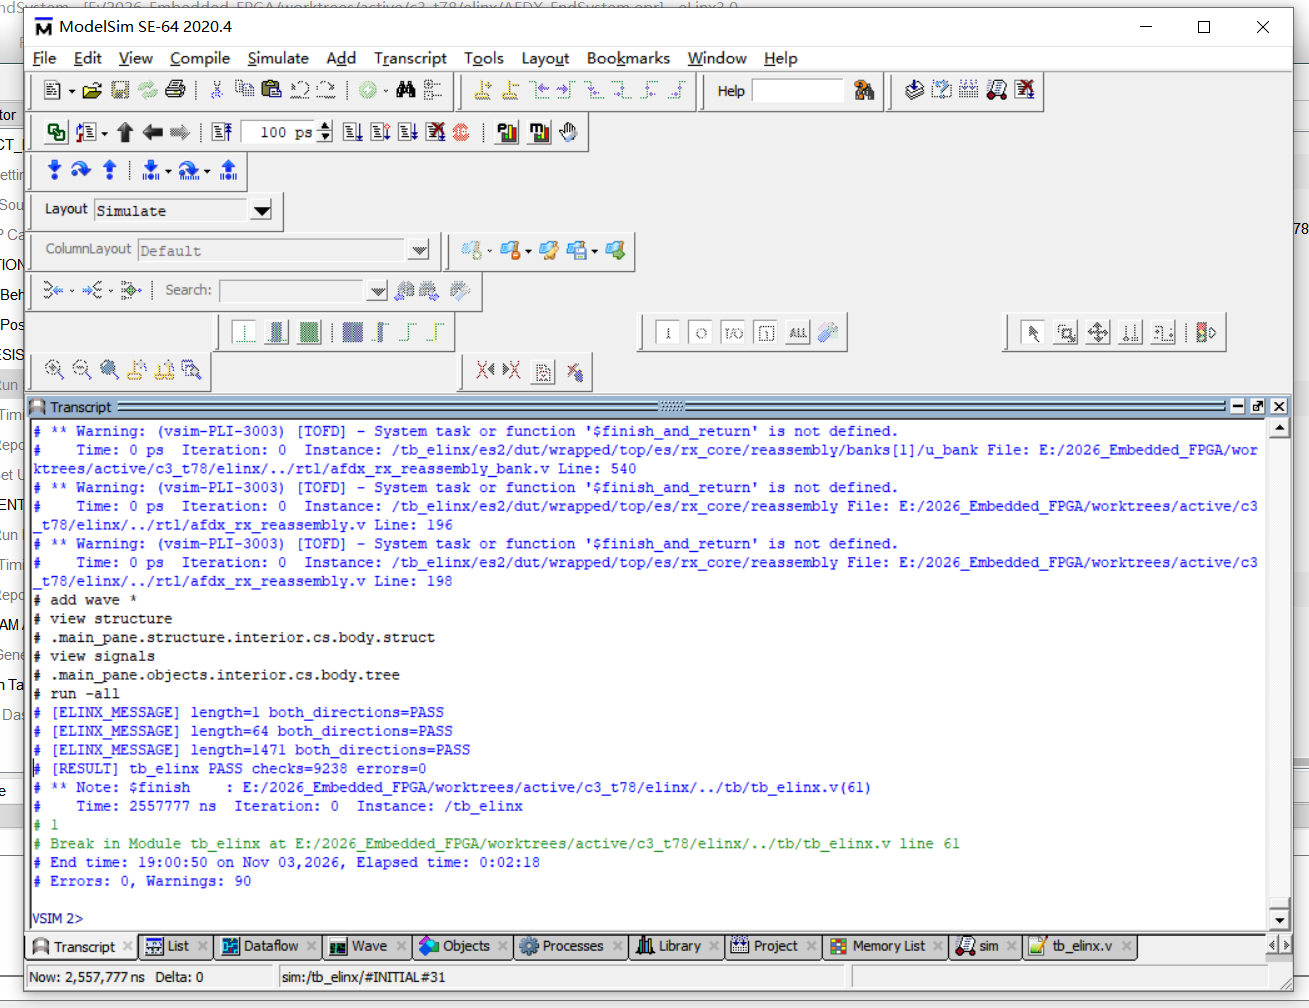
\includegraphics[width=\overviewwidth]{../../sim/wave/png/tb_elinx.png}};
  \draw[draw={rgb,255:red,197;green,80;blue,72},line width=0.6pt]
    (213.54,268.73) rectangle (600.51,355.63);
  \draw[draw={rgb,255:red,197;green,80;blue,72},line width=0.5pt]
    (213.54,268.73) -- (0,212);
  \draw[draw={rgb,255:red,197;green,80;blue,72},line width=0.5pt]
    (600.51,268.73) -- (944,212);
  \begin{scope}[overlay]
    \clip (0,0) rectangle (944,212);
    \node[anchor=south west,inner sep=0] at (-24,-114)
      {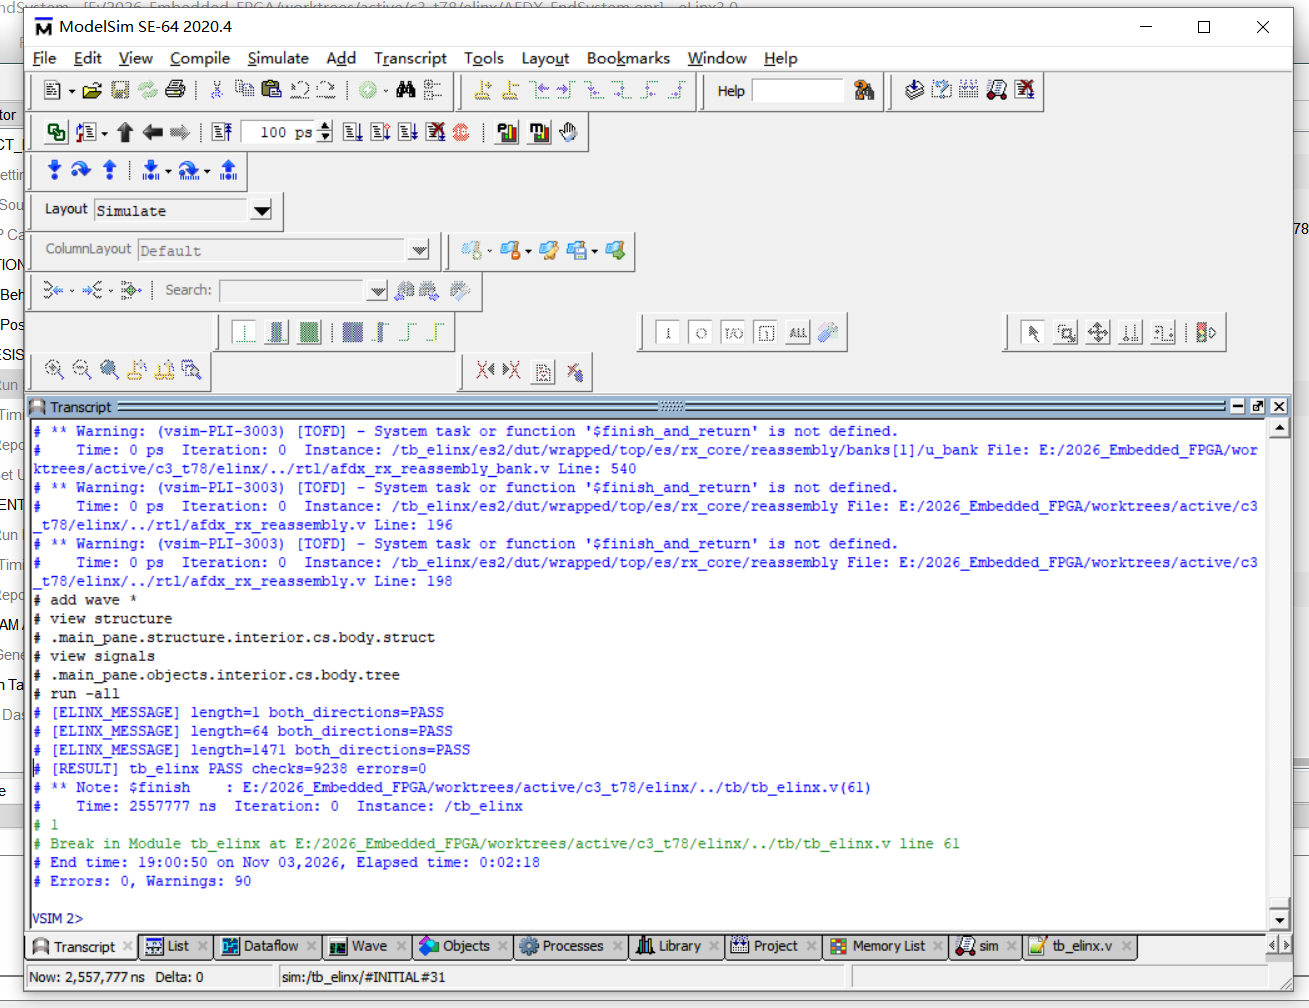
\includegraphics[width=\zoomimagewidth]{../../sim/wave/png/tb_elinx.png}};
  \end{scope}
  \draw[draw={rgb,255:red,197;green,80;blue,72},line width=0.6pt]
    (0,0) rectangle (944,212);
\end{tikzpicture}
\caption{eLinx 3.0.7 调用 ModelSim SE-64 2020.4 运行 \code{tb_elinx} 界面截图及底部 Transcript 日志放大图（\code{checks=9238 errors=0}）}\label{fig:s3_welinx}
\end{figure}

\textbf{评委一键入口 8 项全通过与五功能联合波形成果。}在分片交付版 RTL 上运行无 Python 依赖的评委入口 \code{do sim/run_judge.do}（归档于 \code{sim/reference/judge_result_frag1030.txt}），8 个系统级/性能评审用例全部输出 \code{JUDGE CASE PASS}（总运行时间约 2.3~h，累计完成 \textbf{1,949,513,089 次逐拍/逐字节在线断言检查、0 错误}）。评审用例与逐项检查数见表~\ref{tab:s3_judge}。

\begingroup
\begin{longtable}{@{}>{\raggedright\arraybackslash}p{2.1cm}>{\raggedright\arraybackslash}p{5.5cm}>{\raggedleft\arraybackslash}p{2.5cm}>{\raggedleft\arraybackslash}p{1.9cm}>{\centering\arraybackslash}p{\dimexpr\linewidth-12.0cm-8\tabcolsep\relax}@{}}
\caption{分片交付版评委入口（\code{sim/run_judge.do}）8 项核心评审用例实测汇总表}\label{tab:s3_judge}\\
\longtablehead{5}{\thead{评委用例名} & \thead{考核功能与核心实测指标（\code{judge_result_frag1030.txt}）} & \thead{逐拍/逐字节\newline 断言检查数} & \thead{实测耗时 (s)} & \thead{结论}}
\code{services} & 五项功能（用户收发、IC/RM、SNMP、RTC、615A 加载/卸载）联合自检 & 1,123 & 9.472 & PASS \\
\code{capacity} & 两端各配满 128 TX VL 与 4096 RX VL，抽样验证 0..4095 索引单次去重交付 & 49,924 & 13.669 & PASS \\
\code{snmp} & SNMPv1/v2c 的 Get、GetNext、Set 回写读回及 v2c Trap 启动通知 & 699 & 52.593 & PASS \\
\code{burst77} & 77 条最长帧（1471B）同拍突发排空：\code{queue_clear=983.720 µs} & 530,802 & 16.180 & PASS \\
\code{burst81} & 81 条最长帧（1471B）超规格突发排空：\code{queue_clear=1032.936 µs} & 554,734 & 17.325 & PASS \\
\code{rtc} & SNTP 对时误差：空载 \code{0 ns}，带载 \code{0 ns}，77~VL 满载最大 \code{8 ns} & 10,675,841 & 475.577 & PASS \\
\code{performance} & 77~VL 定长满载双向吞吐 \code{906.136 Mbps/方向}，全消息最大时延 \code{48.600 µs}（d257 为 \code{50.656 µs}），R119 同 VL 抖动 \code{0.008 µs} & 683,408,635 & 3,099.543 & PASS \\
\code{perf_var} & 多 VL 变长（\code{var_fixed/cycle/burst/high}）：\code{var_high} 双向各 \code{904.752 Mbps}、抖动 \code{0.008 µs}；\code{var_cycle} 最大抖动 \code{19.544 µs}（$<50$~µs） & 1,254,291,331 & 4,638.304 & PASS \\
\midrule
\textbf{8 项合计} & \textbf{\code{JUDGE ENTRY PASS cases=8}（Error=0, FAIL=0, RAMCOLL=0）} & \textbf{1,949,513,089} & \textbf{8,322.663} & \textbf{8/8 PASS} \\
\end{longtable}
\endgroup

图~\ref{fig:s3_services_wave} 可对照表中的 \code{services} 用例：从左至右读取 \code{phase}，可依次追踪用户数据、IC 坏序号拦截（\code{ic2=1}）、SNMP、RTC 对时（\code{difference=0 ns}）和 615A 加载成功（\code{status_value=2}）。双网去重计数为 \code{rm1/rm2=29}。

% ModelSim 截图以原始横向坐标对齐信号区与时间轴；只略去菜单及无信号空行。
% 两个位置参数为原图高度比例，分别表示信号区的下裁量、时间轴的上裁量。
\newsavebox{\waveSourceBox}
\newcommand{\waveWindow}[3]{%
  \sbox{\waveSourceBox}{\includegraphics{../../sim/wave/png/#1.png}}%
  \begingroup
  \edef\signalTrim{0pt \the\dimexpr#2\ht\waveSourceBox\relax\space 0pt \the\dimexpr.19\ht\waveSourceBox\relax}%
  \edef\axisTrim{0pt \the\dimexpr.045\ht\waveSourceBox\relax\space 0pt \the\dimexpr#3\ht\waveSourceBox\relax}%
  \edef\signalImage{\noexpand\includegraphics[width=.98\noexpand\linewidth,trim={\signalTrim},clip]{../../sim/wave/png/#1.png}}%
  \edef\axisImage{\noexpand\includegraphics[width=.98\noexpand\linewidth,trim={\axisTrim},clip]{../../sim/wave/png/#1.png}}%
  \vbox{\offinterlineskip
    \hbox{\signalImage}%
    \kern1pt
    \hbox{\axisImage}}%
  \endgroup}

\begin{figure}[H]\centering
\waveWindow{services}{.42}{.85}
\caption{五项功能联合测试（\code{tb_net_services}）的阶段与状态信号（ModelSim）}\label{fig:s3_services_wave}
\end{figure}

\textbf{全设计 \RtlFileCount{} 个 RTL 文件（\DesignUnitCount{} 个设计单元）代码覆盖率成果。}合并 \CovUcdbCount{} 份 UCDB 覆盖率库，全设计语句覆盖率达 \textbf{\CovStmt\%}（\CovStmtCov/\CovStmtTot）、分支覆盖率达 \textbf{\CovBranch\%}（\CovBranchCov/\CovBranchTot）、表达式覆盖率达 \textbf{\CovExpr\%}、FSM 状态覆盖率达 \textbf{\CovFsmState\%}（\CovFsmStateCov/\CovFsmStateTot，其中收发核心与全部高层服务主状态机均为 100.00\%）。各类覆盖率及未覆盖项见表~\ref{tab:s3_cov_sum}。

\begin{table}[H]\centering
\caption{全设计 \RtlFileCount{} 个 RTL 文件（\DesignUnitCount{} 个设计单元）ModelSim 代码覆盖率签核汇总（合并 \CovUcdbCount{} 份 UCDB）}\label{tab:s3_cov_sum}
\begin{tabularx}{\linewidth}{@{}lcccL@{}}
\toprule
\thead{覆盖率类别} & \thead{已覆盖项 / 总项数} & \thead{未覆盖项数} & \thead{实测覆盖率} & \thead{关键模块覆盖特征说明} \\
\midrule
语句覆盖率 (Statement) & \CovStmtCov{} / \CovStmtTot{} & 408 & \textbf{\CovStmt\%} & \code{AFDX_top}、\code{afdx_es}、\code{mac_rx}、\code{rx_core}、\code{tx_core} 等均为 100.0\% \\
分支覆盖率 (Branch) & \CovBranchCov{} / \CovBranchTot{} & 412 & \textbf{\CovBranch\%} & \code{afdx_app_tx} 达 99.81\%，\code{rx_engine} 达 98.96\%，\code{tx_engine} 达 98.38\% \\
表达式覆盖率 (Expression) & \CovExprCov{} / \CovExprTot{} & 745 & \textbf{\CovExpr\%} & \code{afdx_app_rx}、\code{mac_rx}、\code{mgmt_tx}、\code{tx_buf}、\code{tx_core} 均为 100.0\% \\
有限状态机状态 (FSM State) & \CovFsmStateCov{} / \CovFsmStateTot{} & 22 & \textbf{\CovFsmState\%} & 收发核心、MAC 及 RTC/SNMP/615A 服务引擎主状态机均为 \textbf{100.0\%} \\
条件覆盖率 (Condition) & \CovCondCov{} / \CovCondTot{} & 460 & \textbf{\CovCond\%} & 未命中项主要为双口 RAM 原语同址仿真保护与重组极端防卫分支 \\
信号翻转覆盖率 (Toggle) & \countsep{\CovToggleCov} / \countsep{\CovToggleTot} & 23,188 & \textbf{\CovToggle\%} & 未翻转位主要为 32 位异常计数器高 16 位及高序号重组缓存高位线 \\
\bottomrule
\end{tabularx}
\end{table}

\FloatBarrier
\subsection{特性成果}

以下逐项展示作品在五项核心功能、1026/1030 分片重组扩展以及吞吐率、时延、抖动、容量等量化指标上的测试成果与波形记录。

\paragraph{（1）ARINC 664 P7 双网锁步发送、BAG 调度与 $1\text{--}\MaxMessageBytes$~B IPv4 分片重组测试成果}

\textbf{双网同拍发送。}图~\ref{fig:s3_wtx} 先给出从应用口写入到双网 GMII 发送的信号顺序。

\figTest[应用消息与双网同拍发送矢量时序图]{t10_w_tx}{应用消息写入与 A、B 双网同拍发送 RTL 信号波形：(a) 应用口连续写入与调度；(b) 双网 GMII 同拍发出前导码与帧头}{fig:s3_wtx}

图~\ref{fig:s3_cap_tx} 的光标给出实测起点：A、B 两网在 \code{688.572 µs} 的同一时钟沿发出前导码 \code{0x55}。帧头仅第 11 字节源 MAC 接口号不同：A 网为 \code{0x20}，B 网为 \code{0x40}。

\begin{figure}[H]\centering
\waveWindow{tx_dual_1}{.54}{.85}\par\vspace{2pt}
{\footnotesize (a) 应用口写入与 A、B 双网同拍发送总览（光标 \code{688.572 µs} 处双网同步起始）\par}\vspace{4pt}
\waveWindow{tx_dual_2}{.54}{.85}\par\vspace{2pt}
{\footnotesize (b) 双网帧起点局部放大（前导码 \code{55}，源 MAC 网络接口号 A 网 \code{20}、B 网 \code{40}）\par}
\caption{应用消息与 A、B 双网同拍发送的 ModelSim 原始波形截图}\label{fig:s3_cap_tx}
\end{figure}

\textbf{BAG 最小间隔。}图~\ref{fig:s3_cap_bag} 中，同一 VL 相邻两帧的发送起点为 \code{17.132 µs} 与 \code{817.132 µs}。两光标相差 \code{800.000 µs}（100,000 拍），等于配置的 BAG；稳态发送间隔抖动为 \textbf{0.000~µs}。

\begin{figure}[H]\centering
\waveWindow{tx_bag}{.59}{.83}
\caption{同一 VL 两帧发送起点的 BAG 间隔测量（ModelSim）}\label{fig:s3_cap_bag}
\end{figure}

\textbf{8192 字节超长消息 6 分片发送与按序重组实测波形。}针对官方 1030 答疑 R138/R139，图~\ref{fig:s3_cap_frag} 展示了 \code{VL 0x0103} 单条 $8192$~B 最长应用消息的 ModelSim 实测波形（\code{sim/wave/frag.do}）：发送端自动拆分为 6 个 IPv4 分片帧（IP 片偏移依次为 0、1472、2944、4416、5888、7360 字节，前 5 片 \code{MF=1}、末片 \code{MF=0}，图~\ref{fig:s3_cap_frag}c 光标处首片 IP 标志与偏移字段为 \code{20 00}），相邻分片严格间隔 1~ms BAG 从 A、B 双网同拍发出（图~\ref{fig:s3_cap_frag}a）；第 6 片（末片）于 \code{5657.028 µs} 到达后，接收端在 \code{5671.524 µs} 启动连续无反压输出，一次完整交付 \code{8194} 字节（2B 大端 VLID $+$ 8192B 载荷，图~\ref{fig:s3_cap_frag}b），从应用首字节输入（\code{524.768 µs}）至末字节交付结束（\code{5737.076 µs}）总耗时 \code{5212.308 µs}，与输入逐字节 100\% 一致。

\begin{figure}[H]\centering
\waveWindow{frag_1}{.47}{.77}\par\vspace{2pt}
{\footnotesize (a) \code{VL 0x0103} 单条 8192~B 消息拆分为 6 个 IPv4 分片帧（间隔 1~ms BAG）及完整重组交付总览（全程 \code{5212.308 µs}）\par}\vspace{4pt}
\waveWindow{frag_2}{.47}{.77}\par\vspace{2pt}
{\footnotesize (b) 末片到达（\code{5657.028 µs}）后接收端开始连续交付（\code{5671.524 µs}），\code{rx_bytes} 计满 \code{8194} 字节（2B VLID + 8192B 载荷）\par}\vspace{4pt}
\waveWindow{frag_3}{.47}{.79}\par\vspace{2pt}
{\footnotesize (c) 首分片 IP 头字节局部放大（光标 \code{657.252 µs} 处 IPv4 标志与片偏移字段为 \code{20 00}，即 \code{MF=1}、偏移 0）\par}
\caption{8192 字节超长消息 IPv4 6 分片发送与接收端按序重组的 ModelSim 原始波形截图}\label{fig:s3_cap_frag}
\end{figure}

\FloatBarrier
\paragraph{（2）高完整性通信（IC 序号检查、双网 RM 去重与 14 类异常统计）测试成果}

\textbf{IC 序号状态转移与双网独立 PSN 验证。}在用例 RX-03 中，注入序号 7、8（步进 1）、10（步进 2，容忍单帧丢失）均被接纳；注入序号 13（步进 3）被 IC 拒绝但同步更新本网 PSN 为 13，使随后到达的序号 14 立即恢复接纳，而重复注入的序号 14（步进 0）被准确拒绝；A、B 两网 PSN 状态完全独立。其接纳、拒绝及两网独立更新过程见图~\ref{fig:s3_ic_seq}。

\figTest[IC 序号判决与双网独立状态更新验证图]{t03_ic_sequence}{IC 序号完整性判决与双网状态更新实测：(a) 同网连续、丢一帧容忍、跳号拒绝后立即同步及重复帧拦截；(b) A、B 两网独立维护 PSN 状态}{fig:s3_ic_seq}

\textbf{双网去重。}图~\ref{fig:s3_cap_rm} 中，先到的 A 网副本于 \code{3016.844 µs} 交付应用（\code{app_rx_net=0}）。B 网副本晚到 \code{15.784 µs}，在 \code{3032.628 µs} 被共享 RM 模块丢弃，并触发 \code{ev_rm_drop}。

\begin{figure}[H]\centering
\waveWindow{rx_redundancy_1}{.52}{.83}\par\vspace{2pt}
{\footnotesize (a) 先到的 A 网有效副本触发交付事件并输出应用载荷（光标 \code{3016.844 µs}）\par}\vspace{4pt}
\waveWindow{rx_redundancy_2}{.52}{.83}\par\vspace{2pt}
{\footnotesize (b) 晚到的 B 网同序号副本被冗余管理（RM）丢弃并触发 \code{ev_rm_drop}（光标 \code{3032.628 µs}）\par}
\caption{双网冗余副本先到交付与晚到去重的 ModelSim 原始波形截图}\label{fig:s3_cap_rm}
\end{figure}

\textbf{FCS 错误与单网容错。}图~\ref{fig:s3_cap_fcs} 中，A 网 FCS 错帧使 \code{count_a_fcs} 由 0 增至 1，B 网完好副本仍正常交付。主机从配置口读取地址 \code{0x49}，两拍后返回计数值 1。

\begin{figure}[H]\centering
\waveWindow{rx_fcs_error_1}{.45}{.85}\par\vspace{2pt}
{\footnotesize (a) A 网副本检测出 FCS 错误被拒收（\code{count_a_fcs} 增至 1），B 网完好副本正常交付\par}\vspace{4pt}
\waveWindow{rx_fcs_error_3}{.59}{.80}\par\vspace{2pt}
{\footnotesize (b) 主机配置口在 \code{973.404 µs} 读取地址 \code{0x49}，两拍后（\code{973.420 µs}）返回 \code{cfg_rdata=1}\par}
\caption{FCS 错误帧检测、单网容错交付与配置总线读回的 ModelSim 原始波形截图}\label{fig:s3_cap_fcs}
\end{figure}

表~\ref{tab:s3_fault14} 将这一方法扩展到 14 类异常：对照注入位置、样本数与寄存器读回值，可分别核查发送拒绝、接收回退和重组槽回收。

\begingroup
\setlength{\tabcolsep}{3.5pt}
\begin{longtable}{@{}>{\raggedright\arraybackslash}p{2.3cm}>{\raggedright\arraybackslash}p{1.6cm}>{\raggedright\arraybackslash}p{5.5cm}>{\raggedright\arraybackslash}p{\dimexpr\linewidth-9.4cm-6\tabcolsep\relax}@{}}
\caption{收发全通路 14 类异常故障注入与统计寄存器读回验证汇总}\label{tab:s3_fault14}\\
\longtablehead{4}{\thead{异常类别} & \thead{测试用例} & \thead{故障注入方式与样本规模} & \thead{硬件处置行为与配置口寄存器读回结果}}
发送 VL 禁用 & SYS-04 & 向未启用 VL 125 提交 1 条消息 & 拒绝入队、回滚页，\code{0x41 (drop_dis) = 1} \\
发送队列已满 & SYS-04 & 向 \code{qmax=0} 的 VL 127 提交 1 条消息 & 拒绝入队、回滚页，\code{0x42 (drop_full) = 1} \\
发送消息超长 & SYS-04 & 向 \code{max_payload=1} 的 VL 126 提交 18B 消息 & 回滚全部已占页并排空残余字节，\code{0x43 (drop_long) = 1} \\
发送无空闲页 & SYS-04 & 85 条长包占满 255 页后提交 1471/512/1B 消息 & 跨页无页立即退回首占页供 512B 复用，\code{0x44 (drop_nopage) = 2} \\
接收 FCS 错误 & SYS-02 & 改写帧字节，每端每网注入 2 帧（共 8 帧） & \code{mac_rx} 整帧丢弃，每端 \code{0x49/0x51 = 2/2} \\
接收帧长错误 & SYS-02 & 插入截短/超长帧，每端每网 1 帧（共 4 帧） & \code{mac_rx} 整帧丢弃，每端 \code{0x4a/0x52 = 1/1} \\
接收 IP 头错误 & SYS-02 & 插入版本/校验和错误 IP 帧，每端每网 1 帧 & \code{rx_parse} 回退 \code{trial} 指针，每端 \code{0x4b/0x53 = 1/1} \\
接收 UDP 头错误 & SYS-02 & 插入非零错误 UDP 校验和帧，每端每网 1 帧 & \code{rx_parse} 回退 \code{trial} 指针，每端 \code{0x4b/0x53} 累加至 \code{2/2} \\
接收未知 VLID & SYS-02 & 注入未映射 VLID 帧，每端每网 1 帧 & \code{rx_engine} 回退 \code{trial} 指针，每端 \code{0x4c/0x54 = 1/1} \\
接收网络不允许 & SYS-02 & 注入单网禁用副本，每端 A/B 各 1 帧 & \code{rx_engine} 回退 \code{trial} 指针，每端 \code{0x4d/0x55 = 1/1} \\
IC 同网序号重复 & SYS-02 & 四条单向链路各重放 1 帧同 SN 报文 & \code{rx_engine} IC 拦截回退，每端 \code{0x4e/0x56 = 1/1} \\
IC 同网序号乱序 & SYS-02 & 四条单向链路各延后重放旧 SN 报文 & \code{rx_engine} IC 拦截并更新 PSN，每端 \code{0x4e/0x56} 累加至 \code{2/2} \\
接收环形缓冲溢出 & SYS-07 & 环形缓冲缩至 512B，注入 513/1000/1471B 帧 & 空间不足不写入、短帧正常穿插交付，每端 \code{0x4f/0x57 = 3/3} \\
交付队列/重组拒绝 & RX-06/FRAG & 队列缩至 2 项注入 8 帧；注入乱序/缺首片/超 8192B 分片 & 队列满丢弃 1 次、去重 2 次、交付 5 条；异常分片立即回收重组槽 \\
\end{longtable}
\endgroup

\paragraph{（3）SNMP 网络管理、ARINC 615A 软件数据加载与 RTC 时钟同步测试成果}

\textbf{SNMPv1/v2c 查询、设置与 Trap 通知。}通过 \code{pyasn1} 独立验证 36 个 MIB 对象的 v1/v2c Get 精确查询与 GetNext 全表遍历、\code{USER_ID} 读写 Set 与非法写入拦截（只读对象返回 \code{noSuchName=2} 或 \code{notWritable=17}，类型不符返回 \code{badValue=3} 或 \code{wrongType=7}），以及 \code{coldStart} 与 \code{authenticationFailure} 两类 SNMPv2-Trap 报文上报。图~\ref{fig:s3_cap_snmp} 展示了 Get 请求在 \code{525.964 µs} 到达、代理在 \code{538.628 µs}（相距 \code{12.664 µs}）从双网同步发出 GetResponse 的 ModelSim 原始波形。

\begin{figure}[H]\centering
\waveWindow{snmp_get_1}{.54}{.83}\par\vspace{2pt}
{\footnotesize (a) SNMP Get 请求经 A、B 双网到达代理（光标 \code{525.964 µs}）\par}\vspace{4pt}
\waveWindow{snmp_get_2}{.54}{.83}\par\vspace{2pt}
{\footnotesize (b) 代理完成 BER 解码与 MIB 读取后从 A、B 双网同步发出 GetResponse（光标 \code{538.628 µs}，响应耗时 \code{12.664 µs}）\par}
\caption{SNMP Get 请求到达与双网同步响应的 ModelSim 原始波形截图}\label{fig:s3_cap_snmp}
\end{figure}

\textbf{ARINC 615A 软件数据加载与介质定义卸载。}完整通过 1500~B（短末块）与 1536~B（512~B 整倍数补零长末块）上传/卸载、单次丢包超时重传恢复、DATA2 比特翻转 CRC-16 拦截（上报 \code{STATUS=0x0303}）、重传耗尽终止（\code{STATUS=0x0503}）、A4/A3 版本兼容与 A5 非法版本拒绝、RFC 2347 扩展选项忽略等 6 大场景，主机读回的 8~KiB 加载 RAM 与 MDD 回传的 \code{MEMORY.BIN} 均与源文件 100\% 逐字节吻合。图~\ref{fig:s3_w615a} 给出 TFTP 数据块与双网确认时序。

\figTest[ARINC 615A TFTP 数据块传输与确认时序图]{t15_w_615a}{ARINC 615A 目标端 TFTP 数据块接收、双网 ACK 确认与短末块结束传输时序}{fig:s3_w615a}

\textbf{RTC 纳秒级时钟同步。}空载 20 次同步最大误差为 \textbf{\RtcIdle~ns}（评委入口 \code{rtc} 用例在空载与普通带载下均为 \textbf{0~ns}，77~VL 满载下最大误差仅 \textbf{8~ns}；长时带载极限包碰撞下最大误差为 \RtcLoad~ns $=10.788$~µs，小于单帧 12.304~µs 传输时长），并完整通过丢包重发与过期 Originate 防误校测试。请求、应答及校时的先后关系见图~\ref{fig:s3_wrtc}。

\figTest[SNTPv4 时钟同步请求与响应时序图]{t16_w_rtc}{RTC 时钟同步 SNTPv4 客户端请求、服务端回显 Originate 时间戳与本地时钟校准时序}{fig:s3_wrtc}

\FloatBarrier
\paragraph{（4）吞吐率、端到端时延、R97/R119 传输抖动与突发容量量化指标成果}

\textbf{顶层 \code{AFDX_top} 63-VL 声明满载规格与混合分片实测。}在 100~ms 双向双网窗口内，63 条 VL 满载（\code{P1471}）单向去重有效吞吐率达 \textbf{\ThruSixtyThree~Mbps}（双向合计 \textbf{\ThruSixtyThreeBi~Mbps}），最大端到端时延 \textbf{\LatSixtyThreePMax~µs}，同 VL 极差抖动仅 \textbf{0.016~µs}（跨 $1\text{--}1471$~B 五档周期工况最大抖动 $\le\JitSixtyThreePer$~µs）；背靠背两拍轮换突发（\code{B2}）最大时延 \textbf{\LatSixtyThreeBTwo~µs}（$<2000$~µs）、BAG 等待抖动 \textbf{\JitSixtyThreeBTwo~µs}（$<100$~µs）；63~VL 混合单帧与 1472/3000/8192~B 分片长消息（\code{mixed_profile}）双向无损交付 \textbf{12,206 条消息}，0 丢包、0 错包。各工况见表~\ref{tab:s3_perf63}。

\begin{table}[H]\centering
\caption{顶层 \code{AFDX_top} 63-VL 声明满载规格 7 组定长工况与混合分片实测结果（100~ms 双向双网）}\label{tab:s3_perf63}
\setlength{\tabcolsep}{3.5pt}
\begin{tabularx}{\linewidth}{@{}>{\raggedright\arraybackslash}p{2.5cm}>{\raggedleft\arraybackslash}p{2.2cm}>{\raggedleft\arraybackslash}p{2.2cm}>{\raggedleft\arraybackslash}p{2.4cm}>{\centering\arraybackslash}p{1.8cm}>{\raggedleft\arraybackslash}p{1.6cm}>{\centering\arraybackslash}X@{}}
\toprule
\thead{测试场景 / 载荷} & \thead{双向总吞吐\newline (Mbps)} & \thead{最大端到端\newline 时延 (µs)} & \thead{同 VL 最大\newline 抖动 (µs)} & \thead{页池峰值\newline 占用} & \thead{仿真耗时\newline (s)} & \thead{结论} \\
\midrule
\code{P1}（1~B 周期） & 1.008 & 38.440 & 2.016（\code{0x0104}） & 57 / 256 & 740.3 & PASS \\
\code{P17}（17~B 周期） & 17.136 & 34.600 & \textbf{\JitSixtyThreePer}（\code{0x0104}） & 51 / 256 & 751.5 & PASS \\
\code{P256}（256~B 周期） & 258.048 & 41.360 & 0.016（\code{0x010E}） & 16 / 256 & 905.0 & PASS \\
\code{P1024}（1024~B 周期） & 1,032.192 & 65.984 & 0.008（\code{0x0100}） & 14 / 256 & 1,394.5 & PASS \\
\code{P1471}（1471~B 满载） & \textbf{\ThruSixtyThreeBi} & \textbf{\LatSixtyThreePMax} & \textbf{0.016}（\code{0x0100}） & 18 / 256 & 1,418.6 & PASS \\
\code{B1}（1471~B 固定两拍突发） & 1,477.415 & \LatBOne & ---\textsuperscript{*} & 144 / 256 & 1,649.4 & PASS \\
\code{B2}（1471~B 轮换两拍突发） & 1,477.119 & \textbf{\LatSixtyThreeBTwo} & \textbf{\JitSixtyThreeBTwo}（\code{0x0114}） & 156 / 256 & 1,411.6 & PASS \\
\code{mixed_profile}（混合分片） & 60 短 $+$ 3 分片 & 8192B: 5,212.3 & 单帧 $\le 3.360$ & $\le 205 / 256$ & 12,206 条 & PASS \\
\bottomrule
\end{tabularx}
\par\vspace{2pt}\raggedright\footnotesize
注：\textsuperscript{*}\code{B1} 按固定 VL 次序连续注入两帧，3,150 对消息全部通过 BAG 最小间隔与逐字节核对；跨帧抢占下的 BAG 等待抖动由每三相邻 VL 轮换注入次序的 \code{B2} 测量。
\end{table}

\textbf{超规格工况的有效吞吐。}77~VL 与 81~VL 的单向有效吞吐分别为 \textbf{\Thru~Mbps} 与 \textbf{\ThruEightyOne~Mbps}。80~VL 变长高负载（\code{var_high}）下，单向为 \textbf{\ThruVarHigh~Mbps}，双向合计 1809.504~Mbps。图~\ref{fig:s3_thru} 将不同规模与 100~Mbps 赛题门限并列。

\figTest{t20_thru}{不同活跃 VL 规模下的单向有效载荷吞吐率与 100~Mbps 赛题门限对比}{fig:s3_thru}

\textbf{时延与抖动。}内核定长满载（\code{gbe77_d0}）下，单帧提交至末字节交付最大时延为 \textbf{\Lat~µs}，同 VL 抖动仅 \textbf{\JitSameVl~µs}（1 拍）。图~\ref{fig:s3_lat} 按阶段拆解 1471~B 帧的时延；评委入口按全消息统计，\code{max_e2e_us} 为 \textbf{48.600~µs}。

\figTest{t21_lat}{端到端时延与帧长关系及 1471~B 满载帧 3053 拍（24.424~µs）流水拆解}{fig:s3_lat}

\textbf{突发排空。}77 条与 81 条最长帧同拍突发在顶层流接口下的排空时间分别为 \textbf{\BurstSevSeven~µs} 和 \textbf{\BurstEightOne~µs}（评委入口实测 983.720~µs 与 1032.936~µs），均小于 2~ms 门限。内核各工况的分段时延、全消息时延与抖动见表~\ref{tab:s3_perf_core}。

\begingroup
\tablestyle
\setlength{\tabcolsep}{3.2pt}
\begin{longtable}{@{}>{\raggedright\arraybackslash}p{2.2cm}>{\raggedleft\arraybackslash}p{1.8cm}>{\raggedleft\arraybackslash}p{1.6cm}>{\raggedleft\arraybackslash}p{2.3cm}>{\raggedleft\arraybackslash}p{2.3cm}>{\raggedleft\arraybackslash}p{1.8cm}>{\raggedleft\arraybackslash}p{\dimexpr\linewidth-12cm-12\tabcolsep\relax}@{}}
\caption{内核多工况分段时延、全消息时延（分片版评委基准）与抖动实测汇总表}\label{tab:s3_perf_core}\\
\longtablehead{7}{\thead{测试工况} & \thead{单向吞吐\newline (Mbps)} & \thead{$L_\text{tx}$ 基线\newline (µs)} & \thead{$L_\text{rx}$ 首/末\newline (µs)} & \thead{$L_\text{app}$ 基线 / 全消息\newline 最大时延 (µs)} & \thead{R97 / R119\newline 抖动 (µs)} & \thead{发送间隔\newline 偏差 (µs)}}
\code{gbe77_d0} & \textbf{906.136} & 0.312 & 12.360 / 24.120 & 24.432 / \textbf{48.600} & \textbf{0.008} & 0.000 \\
\code{gbe77_d257} & \textbf{906.136} & 0.312 & 12.360 / 24.120 & 26.488 / \textbf{50.656} & \textbf{0.008} & 0.000 \\
\code{gbe81_d0} & \textbf{953.208} & 0.312 & 12.360 / 24.120 & 24.432 / --- & \textbf{0.008} & 0.000 \\
\code{fe10_d0} & 117.680 & 1.880 & 121.648 / 133.408 & 135.288 / --- & 0.000 & 0.000 \\
\midrule
\code{var_fixed_d0} & 57.794 & 0.360 & 12.360 / 24.120 & 24.432 / 48.600 & 0.008 & 0.000 / 0.008 \\
\code{var_cycle_d0} & 70.403 & 12.216 & 12.352 / 24.112 & 24.424 / 48.592 & 9.992 / 19.544 & 6.192 / 12.352 \\
\code{var_high_d0} & \textbf{904.752} & 12.016 & 12.360 / 24.120 & 24.432 / \textbf{48.600} & \textbf{0.008} & 0.000 / 0.016 \\
\code{var_burst_d0} & 57.794 & 21.128 & 12.352 / 24.112 & 32.888 / 63.256 & 0.000 / 0.008 & 0.000 \\
\end{longtable}
\endgroup


% 第四部分：总结 & 第五部分：参考文献
% ======================================================================
% 第四部分：总结 & 第五部分：参考文献
% 严格遵循模板字数限制：
%   4.1 可扩展之处 <= 300 字
%   4.2 心得体会 <= 1000 字
%   第五部分 参考文献 <= 20 篇
% ======================================================================

\section{总结}

\subsection{可扩展之处}

本系统在现有硬件架构上可向三个方向扩展：（1）\textbf{多 VL 并发长包共享重组池：}将当前按槽位固定划分的 $16\times 8$~KiB 重组载荷 RAM 改为基于空闲页链表的共享池化存储，配合可配深度的接收环形缓冲，支持多条 VL 同拍并发注入 $8192$~B 分片长包。（2）\textbf{管理与加载协议子集扩展：}在 \code{CE_DIV=2} 多周期引擎框架下，补充 ARINC 615A 信息操作（LCI）、操作员定义卸载（LNO）及多文件列表批量加载，以及 SNMPv2c \code{GetBulk} 与多变量绑定。（3）\textbf{物理层接口与时间敏感网络融合：}在 GMII 外围增加 RGMII/SGMII 千兆 PHY 跨时钟域弹性桥接逻辑，并结合硬件时间戳通路扩展 IEEE 802.1AS（gPTP）同步协议。

\subsection{心得体会}

在本项目的架构设计与物理收敛过程中，我们重点解决了大容量链路状态存储、超长包分片重组与 125~MHz 静态时序闭环之间的工程矛盾，主要体会如下：

\textbf{第一，片上块 RAM 的分块拓扑必须与物理布线扇出协同规划。}
端系统需同时维护 128 条发送 VL、4096 条接收 VL（含 65,536 项 VLID 映射表）及 16 路 $8192$~B 分片重组上下文。若将 65,536 项 \code{rx_map} 实现为单表，写地址扇出与读出选择树会直接撑破 8.000~ns 时钟周期。我们将 \code{rx_map} 拆分为 32 个子库且每库按高 7 位、低 6 位拆为双写分片（共 64 块 SDP RAM），读侧采用三级寄存或树归并；同时将 \code{rx_cfg} 与 \code{rx_state} 切分为 4~bit/3~bit 窄返回域切片（\code{afdx_rx_table_slice}），将跨阵列长走线转化为固定拍数的短跳流水。

\textbf{第二，大容量 M4K 阵列的保持时间与协议状态机的建立时间需针对性治理。}
引入 $8192$~B 分片重组与顶层 2B-VLID 流包装后，全芯片 CLB 利用率增至 \ClbPct\%、M4K 增至 \Mem{} 块，且需在 8.000~ns 周期上扣除 \ClkUncert~ns 时钟不确定度。布局布线初期，重组载荷 RAM 的空闲写口曾出现短路径保持时间（Hold）违例；我们在 64 条 $8192\times 2$~bit 重组通道的 256 个 M4K 数据输入端前显式插入 128 个 \code{lut_mask="8888"} 写数据隔离 LUT，使布线后最差保持裕量提升至 $+\RoutedHold$~ns。对于包含数十个状态的 SNMP 与 615A 协议引擎，我们未采用易引入握手延迟的异步双时钟 FIFO，而是在单一 125~MHz 时钟下构建 \code{CE_DIV=2} 低扇出使能复制树，将 \countsep{\MulticycleRegs} 个管理触发器约束为 16~ns 多周期路径，配合 \code{tiles_1030.edc} 的 \countsep{\LockedClusters} 个物理簇锁定与 \code{PRES 1.30} 布线参数，实现全芯片 \countsep{\RoutedEndpoints} 个端点 0 违例（净建立裕量 $+\RoutedSetup$~ns）。

\textbf{第三，细粒度流水补偿与独立参考模型比对是保障确定性指标的关键。}
发送组帧器在加入 12 拍 IPv4 校验和准备与输出双缓冲流寄存器后，通过设置 $-8$ 拍提前启动量（\code{START_LEAD_REGISTERED = -8}），使到期帧首前导码准点在允许时刻输出；RTC 模块对 5 拍写回流水固定补偿 40~ns，实现了空载 0~ns 的对时精度。配合独立的 Python 参考模型对 \RegCount{} 项 RTL 回归及 4 类 VQM 门级网表仿真做逐字节核对，多次在迭代早期捕获了跨页回滚与分片偏移边界问题，保证了最终交付工程的可靠性。

% ======================================================================
\section{参考文献}

\begingroup
\small\linespread{1.12}\selectfont
\begin{enumerate}[label={[\arabic*]},leftmargin=2.4em,itemsep=2pt,topsep=4pt]
  \item Aeronautical Radio, Inc. ARINC Specification 664 Part 7: Avionics Full Duplex Switched Ethernet (AFDX) Network[S]. Annapolis: ARINC, 2005.
  \item Aeronautical Radio, Inc. ARINC Report 615A-2: Software Data Loader Using Ethernet Interface[S]. Annapolis: ARINC, 2002.
  \item Aeronautical Radio, Inc. ARINC Report 665-1: Loadable Software Standards[S]. Annapolis: ARINC, 2001.
  \item IEEE Computer Society. IEEE Std 802.3-2018: IEEE Standard for Ethernet[S]. New York: IEEE, 2018.
  \item Postel J. RFC 768: User Datagram Protocol[S]. IETF, 1980.
  \item Postel J. RFC 791: Internet Protocol — DARPA Internet Program Protocol Specification[S]. IETF, 1981.
  \item Sollins K. RFC 1350: The TFTP Protocol (Revision 2)[S]. IETF, 1992.
  \item Malkin G, Harkin A. RFC 2347: TFTP Option Extension[S]. IETF, 1998.
  \item Case J, Fedor M, Schoffstall M, et al. RFC 1157: A Simple Network Management Protocol (SNMP)[S]. IETF, 1990.
  \item Presuhn R. RFC 3416: Version 2 of the Protocol Operations for the Simple Network Management Protocol (SNMP)[S]. IETF, 2002.
  \item Presuhn R. RFC 3418: Management Information Base (MIB) for the Simple Network Management Protocol (SNMP)[S]. IETF, 2002.
  \item Mills D. RFC 4330: Simple Network Time Protocol (SNTP) Version 4 for IPv4, IPv6 and OSI[S]. IETF, 2006.
  \item 全国大学生嵌入式芯片与系统设计竞赛组委会, 中科亿海微电子科技（苏州）有限公司. FPGA 创新设计赛道中科亿海微选题指南（选题一：基于以太网 MAC 总线实现 AFDX）及官方问题汇总（1022/1026/1030 版）[Z]. 2026.
\end{enumerate}
\endgroup


\end{document}
